% =============================================================================
% Technical report: the holding-constraint roadmap (PRM pilot) for the M1
% two-arm bar carry, as implemented in husky_assembly_tamp.motion_planner.
% holding_prm.
%
% Build:  python docs/figures/make_prm_figures.py      (tables, figures, numbers)
%         pdflatex holding_prm_report.tex              (run twice for refs)
% =============================================================================
\documentclass[11pt,a4paper]{article}

% --- page + fonts ------------------------------------------------------------
\usepackage[margin=2.2cm]{geometry}
\usepackage[T1]{fontenc}
\usepackage[utf8]{inputenc}
\usepackage{lmodern}

% --- maths -------------------------------------------------------------------
\usepackage{amsmath,amssymb}

% --- pseudocode ---------------------------------------------------------------
\usepackage{algorithm}
\usepackage{algpseudocode}
\usepackage{caption}

% --- tables, figures, colours, links -------------------------------------------
\usepackage{booktabs}
\usepackage{array}
\usepackage{graphicx}
\usepackage{xcolor}
\usepackage{enumitem}
\usepackage[colorlinks=true,linkcolor=blue!60!black,urlcolor=blue!60!black]{hyperref}

% =============================================================================
% Macros (the same as in cdfm_task_space_birrt_report.tex)
% =============================================================================

% Code identifiers (underscores are typed as-is thanks to \detokenize).
\newcommand{\code}[1]{\texttt{\detokenize{#1}}}

% A line of pseudocode that DIFFERS from the task-space BiRRT is printed in red
% and gets a [P-n] tag at the right margin, pointing to the difference list in
% Section 7.
\definecolor{diff}{RGB}{176,32,32}
\newcommand{\D}[1]{\textcolor{diff}{#1}}
\newcommand{\dtag}[1]{\hfill\textcolor{diff}{\scriptsize\textsf{[#1]}}}

% Pseudocode comments in grey, to the right.
\algrenewcommand{\algorithmiccomment}[1]{\hfill\textcolor{gray}{\footnotesize$\triangleright$ #1}}
\newcommand{\Continue}{\State \textbf{continue}}
\newcommand{\Break}{\State \textbf{break}}

% Non-floating algorithm block that may break across pages.
\newenvironment{algo}[2]{%
  \par\medskip\noindent\rule{\linewidth}{0.8pt}\par
  \captionof{algorithm}{#1}\label{#2}%
  \vspace{-4pt}\noindent\rule{\linewidth}{0.4pt}\par\vspace{-2pt}
  \begin{algorithmic}[1]}%
 {\end{algorithmic}\vspace{-2pt}\noindent\rule{\linewidth}{0.8pt}\par\medskip}

% Long code names in running text: let a line stretch a little rather than
% stick out into the margin.
\setlength{\emergencystretch}{2.5em}

% Maths shorthands.
\newcommand{\R}{\mathbb{R}}
\newcommand{\SE}{\mathrm{SE}(3)}
\newcommand{\norm}[1]{\left\lVert #1 \right\rVert}
\newcommand{\fn}[1]{\textsc{#1}}
\newcommand{\Graph}{\mathcal{G}}

% Table rows written by docs/figures/make_prm_figures.py. The TeX primitive
% input is used because LaTeX's \input cannot start a table row.
\makeatletter\newcommand{\tablerows}[1]{\@@input #1 }\makeatother

% Numbers measured by the pilot (written by docs/figures/make_prm_figures.py).
\newcommand{\PrmLargestBudget}{4000}
\newcommand{\PrmNodesLargest}{4081}
\newcommand{\PrmFreeEdgeShareLargest}{93}
\newcommand{\PrmMedianScoreShort}{7.3}
\newcommand{\PrmMedianScoreLong}{125.2}
\newcommand{\PrmBirrtSolvedStarts}{21}
\newcommand{\PrmBirrtStarts}{807}
\newcommand{\PrmBestGoalLibraryPair}{7}
\newcommand{\PrmBestStartIsLibraryConf}{no}
\newcommand{\PrmBetterBranchStarts}{610}
\newcommand{\PrmReachableStarts}{657}
\newcommand{\PrmSolvedMedianGap}{6.8}
\newcommand{\PrmBestGap}{2.87}
\newcommand{\PrmBestStart}{117}
\newcommand{\PrmBestRouteNodes}{14}
\newcommand{\PrmBestRouteLength}{4.57}
\newcommand{\PrmBestRouteMaxStep}{2.47}
\newcommand{\PrmBestStartPair}{38}
\newcommand{\PrmBestStartTurn}{home}
\newcommand{\PrmBestGoalPair}{5}
\newcommand{\PrmGoalNodes}{14}
\newcommand{\PrmGoalLibraryPairs}{7}
\newcommand{\PrmGoalLibraryPairsFound}{7}
\newcommand{\PrmStartNodes}{17371}
\newcommand{\PrmVerifyRounds}{80}
\newcommand{\PrmLazyChecked}{5461}
\newcommand{\PrmEndpointEdges}{99161}
\newcommand{\PrmExactTwo}{0}
\newcommand{\PrmRoadmapTwo}{0}
\newcommand{\PrmExactFive}{11}
\newcommand{\PrmRoadmapFive}{11}
\newcommand{\PrmExactTen}{34}
\newcommand{\PrmRoadmapTen}{36}
\newcommand{\PrmExactThirty}{245}
\newcommand{\PrmRoadmapThirty}{462}
\newcommand{\PrmRefineEdges}{3329}
\newcommand{\PrmRefineEdgesOk}{2737}
\newcommand{\PrmRefineBranchChange}{372}
\newcommand{\PrmRefineContinuity}{136}
\newcommand{\PrmRefineIk}{65}
\newcommand{\PrmRefineCollision}{19}
\newcommand{\PrmRefineSeconds}{1210}
\newcommand{\PrmRefineRounds}{57}
\newcommand{\PrmExactHorizontal}{164}
\newcommand{\PrmExactBack}{81}
\newcommand{\PrmExactBirrtOverlap}{20}
\newcommand{\PrmExactBestStart}{117}
\newcommand{\PrmExactBestWaypoints}{178}
\newcommand{\PrmExactBestStep}{2.8}
\newcommand{\PrmCheckPaths}{245}
\newcommand{\PrmCheckPassed}{245}
\newcommand{\PrmCheckPassedHorizontal}{164}
\newcommand{\PrmCheckPassedBirrt}{20}
\newcommand{\PrmCheckSeconds}{3607}


\title{A Holding-Constraint Roadmap for the Two-Arm Bar Carry\\
       \large A technical report on the PRM pilot (\texttt{holding\_prm}) and its first measurements}
\author{husky\_assembly\_tamp \texttt{motion\_planner} --- written for Yijiang Huang}
\date{30 September 2026; second version 1 October 2026; third version 2 October 2026}

\begin{document}
\maketitle

\begin{abstract}
\noindent
The task-space BiRRT that plans the M1 two-arm bar carry
(\code{plan_constrained_dual_arm}; see \path{docs/cdfm_task_space_birrt_report.tex})
holds the bar exactly at every waypoint and loses most of its extensions to the
10-degree joint-continuity gate. This report describes the opposite planner,
proposed in the meeting of 29 September 2026 and built as a pilot in
\path{motion_planner/holding_prm/}: a probabilistic roadmap whose nodes hold the
bar exactly, whose edges are straight lines in joint space (so the joints never
jump), and whose edge cost is how far the two tool flanges drift from the bar
along the line. The query searches from a \emph{set} of start configurations to
a \emph{set} of goal configurations, so the start pose and both branch choices
are chosen by the search rather than fixed beforehand. The pseudocode is written
from the code; lines that differ from the BiRRT are printed in \D{red} and tagged
\D{\textsf{[P-n]}}, collected in Section~\ref{sec:diff}. Section~\ref{sec:data}
reports the first measurements on bar B18, goal 2 (the goal whose 807 starts
the BiRRT was run on in full) and on three goals of bar B3.

\smallskip\noindent
\emph{Second version (1 October 2026).} A refinement turns roadmap routes into
paths that hold the bar exactly (Section~\ref{sec:refine}): on B18 goal 2 it gives
an exact path for 34 of the 36 starts within 10\,mm and for 245 starts in all, every
one of which passes the production repair at 2\,mm steps, against 21 starts the
BiRRT solved. New experiments: wider edges (E1), every IK branch at equal draws
(E4), the refinement (E2, E3), a search for better carry poses (E5) and overnight
precomputation (E6). Terms are defined in \emph{Words used} (Section~\ref{sec:words}).

\smallskip\noindent
\emph{Third version (2 October 2026).} The production entry point can now plan on
the roadmap (\code{backend="prm"}), and the roadmap works in scenes that
change from bar to bar (Section~\ref{sec:scene}): a roadmap precomputed with only the
robot, its tools and the bar is placed at the real base pose, and online only the
collisions with the built structure are checked, lazily and in parallel. On bars B1, B3
and B4 of the RobArch demo export it plans the embedded bar carry in every case tried,
including bases parked up to 10\,cm and $5^\circ$ off, and every path passes an
independent production check.
\end{abstract}

\tableofcontents

% =============================================================================
\section{What is being planned, and what changes}
\label{sec:problem}
% =============================================================================

The movement is the same as in the BiRRT report: both UR5e arms of the Husky hold
one bar rigidly and carry it from a carry (home) pose to the approach pose in
front of the structure; the base does not move. The notation is the same too:
$q = (q_L, q_R) \in \R^{12}$ are the twelve arm joints; $G_L, G_R \in \SE$ are
the grasps (the pose of each \code{tool0} flange in the bar frame);
$\mathrm{FK}_L$, $\mathrm{FK}_R$ are the flange forward kinematics. A
configuration holds the bar when both flanges agree on one bar pose,
\begin{equation}
  \mathrm{FK}_L(q_L)\, G_L^{-1} \;=\; \mathrm{FK}_R(q_R)\, G_R^{-1},
  \label{eq:holding}
\end{equation}
and the set $\mathcal{M}$ of such configurations is a six-dimensional surface in
the twelve-dimensional joint space.

\paragraph{The two ways to treat the two constraints.}
A path has to satisfy two things at once: every configuration holds the bar
(Eq.~\ref{eq:holding}), and consecutive configurations are close in joint space
(no joint moves more than $\tau = 10^\circ$ between waypoints). The BiRRT makes
the first one exact and tests the second; its night-1 benchmark measured that
75\,\% of its extensions stop on the second. The roadmap swaps the roles:
\begin{center}
\small
\begin{tabular}{@{}lll@{}}
\toprule
 & task-space BiRRT & holding roadmap (this report) \\
\midrule
holding the bar & exact at every waypoint (IK) & exact at nodes; \emph{measured} along edges \\
joint continuity & tested per waypoint (the gate) & true by construction (straight joint lines) \\
what a failure means & the tree stops growing & the edge costs more \\
answer & a path or nothing & the smallest holding error any path needs \\
\bottomrule
\end{tabular}
\end{center}
The last row is the point of the pilot. The BiRRT cannot tell ``no path exists''
from ``the planner did not find it''. The roadmap always returns a number: the
smallest tolerance on the holding error at which some start connects to some
goal. A small number means near-feasible; a large one means the start and goal
branch sheets are probably not connected.

\paragraph{Only the goal pose is given.}
The export fixes the goal bar pose $T_g$ and nothing else: neither the start
pose nor either configuration. The BiRRT must pick one start configuration and
one goal configuration before it searches (its difference D-9), and a chain of
heuristics does that (goal branch pairing with the home anchors, backward
tracking). The roadmap does not need to choose:
\begin{itemize}[nosep]
  \item the \textbf{goal set} is every collision-free analytical branch pair at
        $T_g$ (up to $8 \times 8$ left-right combinations), each on the
        library's turn and on the home turn (Section~\ref{sec:turns});
  \item the \textbf{start set} is every collision-free branch pair at every
        candidate start pose; the pilot takes the benchmark library's surveyed
        carry poses (807 for B18 goal 2): the three carry anchors
        (horizontal, vertical, on the back), each shifted on a grid of
        $4 \times 4 \times 4$ offsets ($\pm 0.1$ and $\pm 0.3$\,m per axis)
        and rolled about the bar in twelve $30^\circ$ steps, keeping the poses
        that can be held without collision (the library has no yaw variants);
  \item one search runs from a virtual \emph{source}, joined at zero cost to
        every start node, to a virtual \emph{sink}, joined at zero cost to
        every goal node. The cheapest path therefore chooses the start pose,
        the start branch pair and the goal branch pair together, and the report
        says which it chose.
\end{itemize}
Because the grasps are fixed per bar, $\mathcal{M}$ is the same surface for
every goal of a bar: one roadmap per bar and scene can serve all of its goals,
and a query only adds its own start and goal nodes.

\subsection*{Words used in this report}
\label{sec:words}

\begin{center}
\footnotesize
\begin{tabular}{@{}>{\raggedright\arraybackslash}p{2.9cm} >{\raggedright\arraybackslash}p{13.0cm}@{}}
\toprule
word & meaning \\
\midrule
branch pair & One of the (up to $8 \times 8$) ways two arms can hold the bar at one pose: each arm's analytical IK has up to eight solutions (shoulder left/right, elbow up/down, wrist flipped or not), and a branch pair is one left solution with one right solution. Different branch pairs are physically different robot postures. \\
turn & The same posture written with one or more joints shifted by $360^\circ$. Shoulder pan ($\pm 720^\circ$), shoulder lift and the three wrists ($\pm 240$--$270^\circ$) can each reach one angle in two (pan: three) ways. Physically identical; different to a planner that measures raw joint differences. \\
anchor & A configuration the sampler centres its draws on; anchors are also roadmap nodes. They are the home configuration, the goal's branch pairs and a spread of library start configurations, each on up to two turns (Section~\ref{sec:turns}). \\
node budget & The number of \emph{sampled} nodes a build keeps (the \code{--nodes} flag). Anchors come on top. \\
$\beta$ (max branches) & How many of the second arm's IK solutions are kept per draw. $\beta = 1$ keeps only the solution nearest the draw's centre (the default). \\
difficulty class & The benchmark library's label for a start, from a straight-line probe from the goal to the start: \emph{free} (the straight bar move works and is collision-free), \emph{blocked} (it works but collides on the way), \emph{broken} (the IK breaks or jumps on the way). \\
carry anchor & Which of the three carry poses a start was derived from: horizontal (bar along $y$ in front of the robot), vertical (bar along $z$ in front) or back (bar along $x$ over the base). \\
gap (of a node) & The smallest holding tolerance at which this node reaches some goal node through collision-free roadmap edges: the worst edge score on its best route (Section~\ref{sec:query}). A property of the whole route, not of the node's own position. \\
per-start gap & For one start pose, the smallest gap over all its branch pairs and turns. \\
component & A set of nodes joined to each other by collision-free edges; two components have no edge between them. ``Largest'' is the node count of the biggest one. \\
\fn{Collides}$(q)$ & The production full-cell collision check (robot, tools, attached bar, environment); true when $q$ is in collision. \\
\fn{VerifyGaps} & The loop that collision-checks only the edges on each start's best route, searches again, and repeats until those routes are fully checked (Alg.~\ref{alg:lazy}). \\
exact gap & (Section~\ref{sec:refine}) The smallest roadmap tolerance at which a start's route can be turned into a path that holds the bar exactly. \\
\bottomrule
\end{tabular}
\end{center}

% =============================================================================
\section{Where the code lives}
\label{sec:where}
% =============================================================================

\begin{center}
\footnotesize
\begin{tabular}{@{}>{\raggedright\arraybackslash}p{5.3cm} >{\raggedright\arraybackslash}p{3.2cm} >{\raggedright\arraybackslash}p{7.0cm}@{}}
\toprule
\textbf{Function} & \textbf{File} & \textbf{Role} \\
\midrule
\code{holding_violation}, \code{violation_from_tools} & \code{holding.py} & the violation measure (Alg.~\ref{alg:viol}) \\
\code{tool0_world}, \code{build_holding_model} & \code{holding.py} & numpy forward kinematics on the cached arm bases \\
\code{interpolate_confs}, \code{rebranch12} & \code{holding.py} & joint-space lines; moving a configuration onto a $2\pi$ turn \\
\code{draw_driver}, \code{lift_draw}, \code{sample_chunk} & \code{sampling.py} & the node sampler (Algs.~\ref{alg:draw}, \ref{alg:sample}) \\
\code{arm_branches} & \code{sampling.py} & one arm's analytical IK on the cached base \\
\code{expand_bar_pose} & \code{sampling.py} & every collision-free branch pair at a bar pose (Alg.~\ref{alg:expand}) \\
\code{make_collision_fn} & \code{sampling.py} & the production full-cell collision check \\
\code{candidate_pairs}, \code{evaluate_edge} & \code{roadmap.py} & nearest neighbours; measuring one edge (Alg.~\ref{alg:edge}) \\
\code{edge_cost}, \code{Roadmap} & \code{roadmap.py} & the penalised weight; the node and edge tables \\
\code{minimax_to_goals}, \code{route_from} & \code{search.py} & every node's gap to the goal set (Alg.~\ref{alg:minimax}) \\
\code{build_graph}, \code{shortest_between_sets} & \code{search.py} & source/sink search (Dijkstra) \\
\code{lazy_search}, \code{path_report} & \code{search.py} & lazy collision checking (Alg.~\ref{alg:lazy}); path profiles \\
\code{WorkerPool}, \code{init_worker}, \code{task_*} & \code{parallel.py} & worker processes (Section~\ref{sec:parallel}) \\
\code{build_roadmap}, \code{query_roadmap} & \code{pilot.py} & the two drivers (Algs.~\ref{alg:build}, \ref{alg:query}) \\
\code{save_roadmap}, \code{copy_dashboard} & \code{store.py} & files under \path{<root>/prm/}; the dashboard page \\
\code{track_edge}, \code{fine_walk}, \code{track_edge_landing} & \code{tracking.py} & the exact tracker (Section~\ref{sec:refine}) \\
\code{Tracker}, \code{refine_query}, \code{pretrack_roadmap} & \code{refine.py} & exact gaps, assembly, tube rounds; overnight tracking \\
\code{carry_bar_pose}, \code{score_carry_pose} & \code{carry.py} & carry poses and their scores (Section~\ref{sec:e5}) \\
\code{make_collision_fns}, \code{robot_side_signature} & \code{sampling.py} & the collision split and the load signature (Section~\ref{sec:split}) \\
\code{load_carry_movement}, \code{build_scene_cell}, \code{save_scene} & \code{scenes.py} & exported problems; the real scene, cut down for workers \\
\code{plan_on_roadmap}, \code{check_roadmap_fits} & \code{online.py} & the online plan in a live scene (Alg.~\ref{alg:online}) \\
\code{plan_constrained_dual_arm}, keyword \code{backend} & \path{motion_planner/api.py} & the switch between the BiRRT and the roadmap \\
\code{--movement cdfm}, \code{--cdfm-backend} & \path{scripts/headless_bar_}\path{action_planner.py} & planning an exported bar carry with either planner \\
\code{check_file} & \path{scripts/prm_check_solved.py} & independent check of a saved path \\
\code{plan_seeded_birrt} & \path{dual_arm_task_space_rrt/seeded.py} & the BiRRT seeded with a route (imports the core) \\
\code{main} & \path{scripts/prm_pilot.py} & command line: \code{build}, \code{query}, \code{refine}, \code{track}, \code{export}, \code{info} \\
\code{validate}, \code{birrt} & \path{scripts/prm_bridge.py} & the production check; the seeded BiRRT (moves the core's log first) \\
\code{stage1}, \code{starts}, \code{stage2}, \code{pick} & \path{scripts/prm_carry_search.py} & the carry search \\
page & \path{benchmark/dashboard/prm.html}, \path{prm-viewer.js} & the roadmap viewer (Section~\ref{sec:dashboard}) \\
tests & \path{benchmark/tests/test_holding_prm.py} & 31 checks, including one that the package never imports the planner core \\
\bottomrule
\end{tabular}
\end{center}

\noindent
Paths without a folder are in \path{husky_assembly_tamp/motion_planner/holding_prm/}.
What is reused from the rest of the code base:
\code{ssik_inprocess.solve} and \code{ssik_inprocess.fk} (the generated
per-arm solvers and their forward kinematics),
\code{ssik_ik.rebranch_toward_seed}, \code{ARM_SLICE} and \code{ARM_BASE_LINK},
and from the benchmark \code{load_trimmed_problem}, \code{open_scene},
\code{state_with_conf12} and \code{provenance}.

\paragraph{Kept apart from the BiRRT work on purpose.}
Other sessions were editing the planner core, the benchmark runner and the
benchmark dashboard while this was written. The pilot therefore lives in new
files only, writes only under \path{<root>/prm/} (never \path{runs/} or the
batch catalogue \path{runs.json}), has its own command line, and never imports
\path{dual_arm_task_space_rrt/core.py}: that module opens its log file in
\texttt{"w"} mode when imported, which empties a log a running batch may be
writing. Three places where the benchmark reaches the core indirectly are
avoided by writing short local versions: the collision check
(\code{SceneCtx.collision_fn} imports the core for its explain helper), the
library loader (\code{benchmark.library} imports \code{benchmark.sampling},
which imports the core) and the static-site copy. A test runs the import in a
fresh process and asserts no core module is loaded; the log file's size and
time stamp were unchanged across every pilot run.

% =============================================================================
\section{Building blocks}
\label{sec:blocks}
% =============================================================================

\subsection{The holding violation}

\begin{algo}{\textsc{HoldingViolation} --- \texttt{holding\_violation} / \texttt{violation\_from\_tools}}{alg:viol}
\Function{HoldingViolation}{$q$}
  \State $F_L \gets W_L\, \mathrm{fk}_L(q_L)$;\quad $F_R \gets W_R\, \mathrm{fk}_R(q_R)$ \Comment{$W$: arm base in the world, read once per scene}
  \State $F_R^\star \gets F_L\, G_L^{-1} G_R$ \Comment{where the bar placed by the left flange wants the right one}
  \State $F_L^\star \gets F_R\, G_R^{-1} G_L$ \Comment{and the other way round}
  \State $e_p \gets \max\bigl(\norm{p(F_R^\star) - p(F_R)},\ \norm{p(F_L^\star) - p(F_L)}\bigr)$
  \State $e_r \gets \max\bigl(\angle(F_R^\star, F_R),\ \angle(F_L^\star, F_L)\bigr)$ \Comment{angle by $\operatorname{atan2}(\sin, \cos)$}
  \State \Return $(e_p, e_r)$
\EndFunction
\end{algo}

\noindent
Three details. (i) $\mathrm{fk}$ is the ssik artifact's own forward kinematics,
generated from the calibrated URDF like the solver; it takes about
$30\,\mu$s and agrees with PyBullet to $3.4 \times 10^{-7}$ on every
transform entry (measured on 45 library configurations of B3). So the measure
needs no simulator, and the parent process can score whole paths. (ii) Taking
the larger of the two directions makes the measure independent of which arm is
the reference: the two angles are equal, the two distances differ by the lever
arm between the grasps. (iii) The angle of a nearly identity rotation is taken
from both its sine and cosine; an arc-cosine alone loses about half the digits,
which on the dashboard showed as a spurious $0.1^\circ$ error at nodes that hold
the bar exactly. On every library configuration tested (primary goals, goal
branch pairs, starts) the measure returns $10^{-7}$\,m and $2 \times 10^{-7}$\,rad,
four hundred times below the production FK gate.

\paragraph{One number for a tolerance.}
A tolerance is one number $t$ in millimetres. A configuration passes it when
$e_p \le t$\,mm \emph{and} $e_r \le \rho\, t$ degrees, with
$\rho = 0.4^\circ$/mm by default (the ``5\,mm and 2 degrees'' pair of the pilot
plan). Equivalently its \emph{score}
\begin{equation}
  s(q) = \max\bigl(1000\, e_p,\ e_r^{\circ} / \rho\bigr) \quad [\text{mm}]
  \label{eq:score}
\end{equation}
is at most $t$. Edges store $e_p$ and $e_r$ separately, so $\rho$ and $t$ can be
changed without re-measuring anything.

\subsection{Straight lines in joint space, and why continuity is free}

\fn{Interp}$(q_a, q_b; \delta)$ (\code{interpolate_confs}) returns the points of
the straight joint-space line cut into $\lceil \norm{q_b - q_a}_\infty / \delta
\rceil$ equal pieces; the difference is taken on raw joint values, the same
rule as the BiRRT's gate (\code{core.joint_step_deltas}). With $\delta \le
\tau$, every piece of every edge would pass the production continuity gate, so
no path the roadmap returns can contain a branch flip. The tests check the
bound; every path report re-measures the largest step between its dense points.

\subsection{Turns}
\label{sec:turns}

Four of the six UR joint ranges are wider than one turn (shoulder pan
$\pm 2\pi$, shoulder lift $\pm 4.71$, wrists $\pm 4.19$), so one physical
posture can be written as two or three joint vectors $2\pi$ apart. A roadmap
that measures raw joint differences sees these ``twins'' a full turn apart, and
an edge between them would be a full-turn swing. \fn{Rebranch}$(q, r)$
(\code{rebranch12}, which applies \code{ssik_ik.rebranch_toward_seed} per arm)
moves every joint onto the turn nearest a reference $r$ when that stays in
limits. The pilot uses two references: the configuration \emph{as given} (the
library's own turn) and the \emph{home} configuration.

\emph{Which nodes get more than one copy.} A sampled node is stored once: on
the turn nearest the centre of the draw that made it. Only anchors and query
endpoints (start and goal branch pairs) are stored on both turns, and only when
the two copies differ; the query reports which copy a path used. So the
roadmap does not hold every $2\pi$ copy of every node; it holds at most two
copies of the few configurations the search has to start or end at.

This matters in practice: for B18 goal 2, start 0's right shoulder pan
sits at $-319^\circ$ in the library, while the goal's branch pairs sit at
$+50^\circ$ or $+204^\circ$; its home-turn twin is $+41^\circ$, nine degrees
from three of them.

\subsection{Collision}

The check is the production one: copy the template cell state, write the twelve
joints, and let compas\_fab test self-collision, the tools, the attached bar and
the environment with the scene's allowed-collision lists
(\code{make_collision_fn}; the same call as \code{api._build_cfab_collision_fn}).
It costs about 15\,ms and dominates everything else the pilot does: one ssik
solve is 1.8\,ms, one forward-kinematics pair 60\,$\mu$s. A $2\pi$ twin is the
same physical pose, so it is never checked twice.

% =============================================================================
\section{Building the roadmap}
\label{sec:build}
% =============================================================================

\subsection{Anchors}

Draws are centred on \emph{anchors} (\code{make_anchors}): the home
configuration, every collision-free branch pair recorded for the chosen goals
(\code{free_branch_pairs}), and a spread of library starts per goal (40 by
default, picked across the three difficulty classes and the three carry anchors
as the benchmark's \code{select_starts} does), each on its given and its home
turn. Anchors are also inserted as nodes. For B18 goal 2 there are 81: the home
configuration, the goal's 7 branch pairs, and 73 from the 40 anchor starts (40
as given, plus 33 whose home-turn copy differs; the home-turn copies of home and
of the goal pairs coincide with them). A global box spanned by all anchors is
available but off: the 81 anchors of B18 goal 2 span $214^\circ$ to $580^\circ$
per joint (the right shoulder pan the most), i.e.\ the full range, and draws from
that box are the wound-up arms the pilot plan warned about.

\subsection{Sampling: forward kinematics for one arm, IK for the other}

\begin{algo}{\textsc{DrawDriver} --- \texttt{draw\_driver}}{alg:draw}
\Function{DrawDriver}{mode, driver}
  \State $a \gets$ uniform anchor index;\quad $c \gets$ anchor$[a]$ \Comment{$c$: the 12-joint centre of the draw}
  \If{mode $=$ \code{anchor_box}} $q_d \sim \mathcal{U}(c_d \pm m)$ \Comment{$m = 90^\circ$ per joint}
  \ElsIf{mode $=$ \code{anchor_gauss}} $q_d \sim \mathcal{N}(c_d, \sigma^2)$ \Comment{$\sigma = 30^\circ$}
  \ElsIf{mode $=$ \code{anchor_line}}
    \State $b \gets$ an anchor of a different role (start $\leftrightarrow$ goal) \Comment{a start--goal line when possible}
    \State $c \gets c + u\,(\text{anchor}[b] - c)$, $u \sim \mathcal{U}(0,1)$;\quad $q_d \sim \mathcal{N}(c_d, \sigma_\ell^2)$ \Comment{$\sigma_\ell = 10^\circ$}
  \EndIf
  \State \Return (clip($q_d$, limits), $c$, $a$)
\EndFunction
\end{algo}

\begin{algo}{\textsc{SampleChunk} --- \texttt{sample\_chunk} / \texttt{lift\_draw}}{alg:sample}
\Function{SampleChunk}{seed, $k$, $n$}
  \State rng $\gets$ \code{SeedSequence}(seed, $k$) \Comment{chunk $k$ gives the same nodes on any worker}
  \For{$i = 1 \dots n$}
    \State driver $\gets$ L if $(kn + i)$ even else R;\quad other $\gets$ the other arm \Comment{both arms drive equally often}
    \State mode $\sim$ mix;\quad $(q_d, c, a) \gets$ \fn{DrawDriver}(mode, driver) \Comment{default mix 0.2 / 0.3 / 0.5}
    \State \D{$T \gets \mathrm{FK}_{\text{driver}}(q_d)\, G_{\text{driver}}^{-1}$} \Comment{the bar pose this arm implies}\dtag{P-1}
    \State \D{$B \gets$ \fn{IK}$_{\text{other}}(T\, G_{\text{other}};\ \text{seed} = c_{\text{other}},\ \text{rescue off})$} \Comment{re-branched to $c$, nearest first}\dtag{P-8}
    \State $B \gets B[1{:}\beta]$ \Comment{$\beta = 1$: the branch nearest the centre}
    \For{$q_o \in B$}
      \State $q \gets (q_d, q_o)$;\quad \textbf{assert} \fn{HoldingViolation}$(q) \le 10^{-4}$ \Comment{a failure stops the build}
      \If{\textbf{not} \fn{Collides}$(q)$} keep $q$ with (mode, driver, $a$, geometry) \EndIf
    \EndFor
  \EndFor
\EndFunction
\end{algo}

\noindent
Each draw gives the second arm up to eight IK solutions; $\beta$ is how many
of them become nodes, nearest the draw's centre first. Keeping only the nearest
($\beta = 1$) was a measured choice. On a small smoke roadmap (bar B3) with a
node budget of 300 sampled nodes, keeping every solution split the roadmap into
103 components: the second arm's median distance to the anchor was
$182^\circ$, i.e.\ most kept nodes were flipped elbows or wrists that sit far
from every other node and join nothing. With $\beta = 1$, the same budget of
300 nodes gave 44 components. The B18 comparison at 2000 nodes is in
Table~\ref{tab:ablation}, and Section~\ref{sec:e4} repeats it with the same
number of draws instead of the same number of nodes. Other branch sheets are
still represented, because every branch pair of the goal is an anchor and draws
around an anchor are seeded from that anchor.

\subsection{Edges}

\begin{algo}{\textsc{EvaluateEdge} --- \texttt{evaluate\_edge}}{alg:edge}
\Function{EvaluateEdge}{$q_a$, $q_b$}
  \State $(e_p^{\max}, e_r^{\max}, t^\star) \gets \max$ of \fn{HoldingViolation} over \fn{Interp}$(q_a, q_b; \delta_v)$ \Comment{$\delta_v = 2.5^\circ$, nearly free}\dtag{P-3}
  \State $P \gets$ interior points of \fn{Interp}$(q_a, q_b; \delta_c)$ \Comment{$\delta_c = 10^\circ = \tau$}\dtag{P-2}
  \For{$j$ \textbf{in} bisection order of $P$} \Comment{middle first, then quarters, \dots}
    \If{\fn{Collides}$(P_j)$} \Return (free $=$ false, $t_{\text{collide}} = j/|P|$, $e_p^{\max}$, $e_r^{\max}$) \EndIf
  \EndFor
  \State \Return (free $=$ true, $e_p^{\max}$, $e_r^{\max}$, $t^\star$, $\norm{q_b - q_a}_2$, $\norm{q_b - q_a}_\infty$)
\EndFunction
\end{algo}

\noindent
Candidate pairs (\code{candidate_pairs}) are each node's $k = 10$ nearest
neighbours in the largest-joint-move metric (a \code{cKDTree} with $p = \infty$)
no further than $90^\circ$, symmetrised and sorted so the work splits into the
same chunks every time. The violation is measured four times more finely than
collision because it costs two forward-kinematics calls per point; collision is
checked at the continuity step, which is also what the production gate would
look at. The end nodes are already known to be free.

\begin{algo}{\textsc{BuildRoadmap} --- \texttt{build\_roadmap}}{alg:build}
\Function{BuildRoadmap}{bar, goals, $N$}
  \State start the worker pool (one scene per process) \Comment{Section~\ref{sec:parallel}}
  \State anchors $\gets$ \code{make_anchors}(goals); insert the collision-free ones as nodes
  \While{fewer than $N$ sampled nodes kept}
    \State issue chunks $k, k{+}1, \dots$ of \fn{SampleChunk} in parallel \Comment{round size from the measured yield}
  \EndWhile
  \State keep the first $N$ sampled nodes in chunk order \Comment{same nodes for any worker count}
  \State pairs $\gets$ \code{candidate_pairs}(nodes, $k$, radius)
  \State edges $\gets$ \fn{EvaluateEdge} on every pair, in parallel (collision skipped with \code{--lazy})
  \State save \path{roadmap.json.gz} and \path{config.json}; add the run to \path{prm/index.json}
\EndFunction
\end{algo}

% =============================================================================
\section{Querying the roadmap}
\label{sec:query}
% =============================================================================

\subsection{Endpoints}

\begin{algo}{\textsc{ExpandBarPose} --- \texttt{expand\_bar\_pose}}{alg:expand}
\Function{ExpandBarPose}{$T$, references}
  \State $B_L \gets$ \fn{IK}$_L(T G_L)$;\quad $B_R \gets$ \fn{IK}$_R(T G_R)$ \Comment{all branches, rescue on (one-off solve)}
  \For{$(q_L, q_R) \in B_L \times B_R$} \Comment{up to 64 pairs}\dtag{P-5}
    \If{\fn{Collides}$(q_L, q_R)$} \Continue \EndIf
    \For{(name, $r$) \textbf{in} references} \Comment{given: the library configuration; home}
      \State $q' \gets$ \fn{Rebranch}$((q_L, q_R), r)$; merge with an equal $q'$ already listed, adding the name
    \EndFor
  \EndFor
  \State \Return every distinct $q'$ with its pair index and turn names
\EndFunction
\end{algo}

\noindent
The goal pose and every chosen start pose are expanded in parallel, one pose
per task. Each start node carries five labels, all different things (see
\emph{Words used}): its start index (which library start pose), carry anchor
(horizontal, vertical or back), difficulty class (free, blocked or broken:
the library's straight-line probe), branch-pair index (which of the up to 64
postures at that pose) and turn (which $2\pi$ copy of that posture); plus
whether it is the library's own configuration. The expansion must find the library's \code{free_branch_pairs}
again (they are the same pairs, solved by the same solver); a test checks this on
the smoke goal, every query records the count, and every B18 query found all 7
of goal 2's pairs.

\subsection{The gap of every node}

\begin{algo}{\textsc{MinimaxToGoals} --- \texttt{minimax\_to\_goals}}{alg:minimax}
\Function{MinimaxToGoals}{$\Graph$, goal set}
  \State weight every usable edge by its score $s$ (Eq.~\ref{eq:score}); join a sink to every goal node at 0
  \State $M \gets$ minimum spanning tree of $\Graph$ (Kruskal)
  \State gap(sink) $\gets 0$
  \For{each tree edge $(u, v)$ in breadth-first order from the sink}
    \State gap$(v) \gets \max(\text{gap}(u), s_{uv})$;\quad parent$(v) \gets u$
  \EndFor
  \State \Return gap, parent \Comment{gap $= \infty$ for nodes not joined to any goal}
\EndFunction
\end{algo}

\noindent
In a minimum spanning tree, the tree path between two nodes has the smallest
possible largest edge of any path between them. With the sink joined to the goal
set, one tree gives \emph{every} node its \emph{gap}: the smallest tolerance at
which a chain of free edges joins it to some goal node, and the next node on
that chain. The best start is the start node with the smallest gap; a start
index's gap is the smallest gap over its branch pairs and turns. On the
dashboard any clicked node's best route to the goals is simply followed through
the parent pointers.

\subsection{Lazy collision checking}

Expanding every start of a goal gives thousands of endpoint nodes and tens of
thousands of candidate endpoint edges; checking all of them for collision would
cost more than the roadmap. The query measures the holding error of every
endpoint edge (cheap) but checks collision only where it decides an answer.
\fn{VerifyGaps} does this for the gaps: it first computes every node's gap as
if all unchecked edges were free, collision-checks only the edges on each
start's best route, drops the ones that collide, and repeats until every
start's best route consists of checked, free edges.

\begin{algo}{\textsc{VerifyGaps} and \textsc{LazySearch} --- \texttt{query\_roadmap} / \texttt{lazy\_search}}{alg:lazy}
\Function{VerifyGaps}{}
  \Repeat
    \State (gap, parent) $\gets$ \fn{MinimaxToGoals} with unchecked edges assumed free \dtag{P-7}
    \State $U \gets$ unchecked edges on the route (via parent) of each start index's best node
    \State collision-check $U$ in parallel; mark the colliding ones blocked
  \Until{$U = \varnothing$}
\EndFunction
\Statex
\Function{LazySearch}{find\_path}
  \Repeat
    \State $P \gets$ find\_path(edges free or unchecked) \Comment{filtered or penalised Dijkstra, source $\to$ sink}
    \State $U \gets$ unchecked edges of $P$; check them in parallel; mark the colliding ones
  \Until{$P = \textsc{None}$ \textbf{or} $U = \varnothing$}
  \State \Return $P$
\EndFunction
\end{algo}

\noindent
Both loops are exact, not approximations. Assuming unchecked edges free can only
lower a gap or shorten a path; when the deciding route comes back with every
edge checked and free, nothing cheaper exists in the true graph, since the true
graph is a subset of the optimistic one. For the best node of each start index
this makes the gap exact; the gaps of other nodes stay optimistic lower bounds
and are only used for colouring.

\subsection{The questions asked}

\begin{algo}{\textsc{QueryRoadmap} --- \texttt{query\_roadmap}}{alg:query}
\Function{QueryRoadmap}{roadmap, goal, starts, tolerances}
  \State goal nodes $\gets$ \fn{ExpandBarPose}($T_g$, \{given: primary, home\}) \dtag{P-5}
  \State start nodes $\gets \bigcup_s$ \fn{ExpandBarPose}($T_s$, \{given: $q_s$, home\}); reuse roadmap nodes at the same $q$
  \State endpoint edges $\gets$ \fn{EvaluateEdge} without collision on each new node's $k$ nearest (radius $90^\circ$)
  \State \fn{VerifyGaps}() \Comment{per-start gap, exact}
  \State best $\gets$ start node of smallest gap; report its route (the minimax route)
  \State report the shortest path within the best gap (\fn{LazySearch}, filtered at gap)
  \For{$t$ \textbf{in} tolerances ($2, 5, 10, 30$\,mm)} \dtag{P-6}
    \State \emph{filtered}: \fn{LazySearch} over edges with $s \le t$, weight $= \norm{\Delta q}_2$
    \State \emph{penalised}: \fn{LazySearch} over all free edges, weight $= \norm{\Delta q}_2 + w \max(0, s/t - 1)$
    \State starts connected $\gets \#\{$start indices with gap $\le t\}$
  \EndFor
  \State save the query: endpoint tables, final edge verdicts, every node's gap and parent, the paths with their dense profiles
\EndFunction
\end{algo}

\noindent
Each path report stores the node list, the start and goal it used (start index,
carry anchor, branch pair, turn; goal pair, turn), the dense joint path at
$\delta_v$, the holding error at every dense point, where the worst point sits,
and the largest joint step between dense points (at most $\delta_v$ by
construction). The penalised weight uses $w = 10$: going one tolerance over
costs as much as ten radians of joint travel.

% =============================================================================
\section{Refinement: from a roadmap route to a path that holds the bar exactly}
\label{sec:refine}
% =============================================================================

A roadmap route within a tolerance $t$ is a chain of straight joint-space edges
whose holding error stays under $t$; its nodes hold the bar exactly, the points
between them do not. The refinement turns such routes into paths that hold the
bar \emph{exactly}, at every waypoint, without giving up continuity. It is built
in four layers, each tried only where the one before it fails (code:
\path{holding_prm/tracking.py}, \path{refine.py}; \path{scripts/prm_bridge.py}
and \path{dual_arm_task_space_rrt/seeded.py} for the parts that use the planner
core).

\subsection{Tracking one edge exactly}

\begin{algo}{\textsc{TrackEdge} --- \texttt{tracking.track\_edge}}{alg:track}
\Function{TrackEdge}{$q_a$, $q_b$; seed $s$ (default $q_a$)}
  \State knots $k_0 = q_a, \dots, k_m = q_b$ on the joint line, every $2.5^\circ$ of largest joint move
  \State $T_i \gets$ the bar pose halfway between the two arms' bar poses at $k_i$ \Comment{exact at $q_a$, $q_b$}
  \State waypoints: $T_i \to T_{i+1}$ cut into $\lceil \max(d/\Delta_p,\ \theta/\Delta_r) \rceil$ equal pieces \Comment{the BiRRT's rule, $\Delta_p = 1$\,cm, $\Delta_r = 0.025$\,rad}
  \State $p \gets s$
  \For{each waypoint bar pose $T$, with $g$ = the joint line's configuration at the same place}
    \For{each arm}
      \State $B \gets$ \fn{IK}$(T G)$, every branch moved onto $p$'s turn \Comment{rescue off}
      \State $B' \gets \{q \in B : \norm{q - p}_\infty \le 10^\circ\}$; \textbf{if} empty: \Return continuity (or IK) failure
      \State take the $q \in B'$ nearest $g$ \Comment{$B'$ usually has one element}
    \EndFor
    \If{the step from $p$ moves some joint more than $0.5^\circ$}
      \State re-walk it at 2\,mm / 0.002\,rad, nearest branch each step; keep where it arrives \Comment{\fn{FineWalk}}
    \EndIf
    \State $p \gets$ the solved configuration; append it
  \EndFor
  \State \fn{Collides} on the solved waypoints, middle first; \Return the waypoints or the failure and where
\EndFunction
\end{algo}

\noindent
The roadmap's configurations are only seeds and a yardstick: the first solve is
seeded from the start node, every later one from the waypoint solved just
before it (as the BiRRT extension does), and nothing requires the chain to
reproduce a stored node. The joint line's configuration $g$ only breaks ties:
near a straight elbow or a straight wrist two branches can both lie within the
gate of the previous waypoint, and then the one on the roadmap's side is taken.
The waypoints hold the bar to $10^{-7}$\,m, because each one is an IK solution
of both arms at one bar pose.

\paragraph{Why (nearly) every step is walked again finely.} The gate cannot tell
a large honest step from a hop between branches: near a straight elbow or wrist
the two branches can be closer than $10^\circ$. The production check found this
in four rounds:
\begin{enumerate}[nosep]
  \item With 1\,cm steps alone, 31 of 38 exact paths were walked by the production
        repair to the goal pose but arrived on another branch. On the best path
        (start 117) the cause was one $9.6^\circ$ step at a $4.8^\circ$ elbow where
        the chain had hopped to the mirror branch; walked at 2\,mm the arm stays on
        its branch and arrives $9.4^\circ$ away.
  \item Re-walking every step above $2^\circ$ at the production's resolution
        (\fn{FineWalk}: bar frame interpolated at 2\,mm and 0.002\,rad, warm IK
        nearest the previous solution, the gate at every step) raised the pass
        rate to 217 of 244 (89\,\%). All 27 failures were collisions, and none
        was a collision of our own waypoints or of the joint lines between them:
        the production walk had left our path at a smaller hop ($4^\circ$ at a
        $2^\circ$ elbow, $8^\circ$ at a $4^\circ$ elbow) on an edge that had been
        tracked from its far end, and only collided further on.
  \item Near such a point, which branch a walk keeps depends on the direction it
        walks in, so waypoints walked from one end and read backwards are not what
        a walk from the other end gives. Re-walking every step above $0.5^\circ$
        finely and tracking each edge in both directions (each direction keeping
        its own waypoints; a route uses an edge only in a direction that worked)
        left 25 failures in 268, again all collisions.
  \item The remaining hops sat at nodes: an edge's chain had arrived within the
        gate of the shared node but on the mirror elbow solution ($-4.3^\circ$
        against the node's $+4.1^\circ$), and the next edge started from the
        node's own solution. Now an edge counts as tracked only when its chain
        ends on its node's own solution (next paragraph).
\end{enumerate}
\fn{FineWalk} uses IK only (two solves per 2\,mm step), so it roughly doubles
the cost of tracking; collision is still checked at the 1\,cm waypoints.

\paragraph{When an edge counts as tracked.} A path is one chain, so where two
edges meet, the next edge's chain must start where the arriving one ended. The
next edge was tracked from the shared node, so an edge counts as tracked when
its chain, started at one node, ends on the other node's own IK solution (both
are solves at that node's bar pose, so they agree to $10^{-9}$ when they are the
same solution). ``Within the $10^\circ$ gate'' is not enough: near a straight
elbow the mirror solution can be closer than that, and switching between two
solutions at one pose is a branch flip no walk makes. (A seeded chain that
continues a route from wherever it is need not end on the node; the route's next
edge is then continued from there in the same way.) Usually an edge's chain does
end on its node. It does not when the edge's joint line passes
through a fully stretched elbow, where the two elbow branches meet: the
corrected path, halfway between what the two arms imply, stays short of that
point, so the chain cannot cross over and arrives on the mirror branch,
25--$35^\circ$ from the node on the elbow joint. This happened to 4 of 60
random B18 edges; neither finer steps nor the tie-break changed it. Such a
direction is marked as \emph{changing branch}; the edge stays usable in the
other direction if that one arrives.

\subsection{Exact gaps: tracking routes until they all track}

\begin{algo}{\textsc{ExactGaps} --- \texttt{refine.Tracker.exact\_gaps}}{alg:exactgaps}
\Function{ExactGaps}{query graph, starts within 30\,mm}
  \State every collision-usable edge is \emph{untracked} and assumed trackable
  \Repeat
    \Repeat
      \State (gap, parent) $\gets$ \fn{MinimaxToGoals} over the edges not known to fail
      \State $U \gets$ untracked edges on each start's best route; \fn{TrackEdge} them in parallel; mark failures
    \Until{$U = \varnothing$}
    \State assemble each start's route into one chain \Comment{below}
    \State where a chain cannot continue: drop the edge that left the roadmap's branch
  \Until{every route assembles}
  \State \Return each start's \emph{exact gap} (its route's gap) and its exact path
\EndFunction
\end{algo}

\noindent
This is \fn{VerifyGaps} with ``track it'' in place of ``collision-check it'',
and exact for the same reason: tracking can only remove edges, so a route whose
edges all track is the best route the graph has left. The \emph{exact gap} of a
start is therefore the smallest roadmap tolerance at which this roadmap yields
a path that holds the bar exactly. \emph{Assembly} joins a route's tracked
edges into one chain and checks the gate at every node. Because every tracked
edge arrives within the gate of both its nodes, this normally just works; where
it does not (an edge tracked from its far end arrives a few degrees from the
node), the next edge is tracked again, seeded from where the chain actually
is, and if that fails the offending edge is dropped and the routes are searched
again.

\subsection{Tube draws around a route (way 2)}

For a start whose exact gap is above the target (10\,mm), new nodes are drawn
around its current best route: a point is picked on the route's joint lines
(points on edges over the target, or that failed to track, four times as often),
the driving arm's joints are drawn from a Gaussian of $5^\circ$ around it, and
the other arm is solved as in Alg.~\ref{alg:sample}. The new nodes join their
10 nearest neighbours within $30^\circ$ (holding error measured; collision left
to the tracker), and \fn{ExactGaps} runs again on the enlarged graph. Up to
three rounds, stopping after two rounds in a row with no start improving.

\subsection{A BiRRT seeded with the route (way 1)}

For a start the roadmap brings within 30\,mm but that has no exact path even
after the tube rounds (the 24 with the smallest roadmap gaps are tried), a
task-space BiRRT bridges the failed edges of its original roadmap route
with the production planner's own extension (\code{core.extend_toward}: warm
IK, the $10^\circ$ gate, the full collision check). Its two trees do not start
at the two ends: tree A is the chain of exact waypoints from the start up to
the first failed edge, tree B the chain from the goal back to the last failed
edge. Random targets are bar poses in a tube around the route's bar poses
(5\,cm and $8.6^\circ$ spreads; poses on failed edges four times as often),
with a 10\,\% chance of aiming at the other tree's tip. A control run starts
the trees from the two ends only, to separate the value of the exact chains
from that of the tube.

\subsection{The production check}

Every stored exact path is finally re-solved by the production repair
(\code{core.repair_joint_path}) at the benchmark's fine resolution (2\,mm and
0.002\,rad bar steps), with the production solver, gate and collision check.
A path that passes is one the production planner would accept as is.

% =============================================================================
\section{Running it in parallel}
\label{sec:parallel}
% =============================================================================

Sampling, edge checking and endpoint expansion are the same small computation
thousands of times over, each independent. \code{WorkerPool} is a
\code{ProcessPoolExecutor} with the \code{spawn} start method (the pattern of
the benchmark's parallel library build); each worker opens its own headless
PyBullet scene once, in its initializer, and keeps it. Processes, not threads:
\code{pybullet_planning} keeps one global simulation and the collision check
writes joints into it. Tasks and results are plain lists, so nothing that
cannot cross a process boundary on Windows ever does; each edge task carries the
configurations it needs (64 edges, about 12\,kB). Results are re-sorted by chunk
index, so the roadmap is the same for any worker count, and the parent never
opens a scene: it does the nearest-neighbour search, the graph searches and the
file writing. A worker that dies surfaces as a broken pool at once. Each
worker sets \code{OMP_NUM_THREADS=1} so six or eight of them do not fight a
running benchmark batch for cores; the default is six workers, eight were used
for the runs below while no batch was running.

% =============================================================================
\section{Storage and the dashboard}
\label{sec:dashboard}
% =============================================================================

\begin{center}
\footnotesize
\begin{tabular}{@{}lp{10.5cm}@{}}
\toprule
file & contents \\
\midrule
\path{prm/index.json} & every roadmap run (only this tool writes it) \\
\path{prm/<run>/config.json} & settings, anchors, tallies per phase, timings, provenance (git state of every repository, versions, ssik artifacts) \\
\path{prm/<run>/roadmap.json.gz} & holding model; nodes as columns (configuration, both flange positions, their midpoint, bar pose, violation, kind, sampling mode, driver, anchor); edges as columns (ends, lengths, checked, free, where it collides, worst position and rotation error, where) \\
\path{prm/<run>/queries/<tag>.json.gz} & endpoint nodes and edges, the final verdict of every edge, every node's gap and parent, the paths with dense profiles, the per-start table \\
\path{prm/<run>/dashboard/} & the page (\path{prm.html}, also as \path{index.html}) with the shared scripts \\
\bottomrule
\end{tabular}
\end{center}

\noindent
The page reuses the benchmark dashboard's robot viewer, loaders and charts
without changing them. Each node is a ball at the midpoint of the two flanges
(grey sampled, purple anchors, green starts, blue goals; or coloured by gap).
Balls are instanced meshes registered in the viewer's list of pickable clouds,
so the existing click handler reports them. Clicking a ball poses the robot,
lists the twelve joints, the node's role (anchor, which start or goal pair, which
turn), its gap, and its edges sorted by holding error, each with a ``walk''
button. Edges are drawn green within the tolerance slider's value, amber up to
three times it, red beyond. The best route of the clicked node is drawn and can
be stepped through; at every step the page recomputes the holding error from the
posed flanges, and a second, orange bar placed by the right flange shows the
drift. Serve the data root and open \path{http://localhost:8000/prm/<run>/dashboard/}.

\paragraph{How to run it.} From the repository root, with \code{HUSKY_BENCH_ROOT}
set to the benchmark data root (PowerShell shown):
{\footnotesize
\begin{verbatim}
.venv\Scripts\python.exe scripts\prm_pilot.py build --name B18_g2_n4000 --library cdfm_v1 `
    --bar B18 --goals 2 --anchor-starts 40 --nodes 4000 --workers 8
.venv\Scripts\python.exe scripts\prm_pilot.py query --name B18_g2_n4000 --goal 2 `
    --starts all --tag all
.venv\Scripts\python.exe scripts\prm_pilot.py export --name B18_g2_n4000
.venv\Scripts\python.exe scripts\prm_pilot.py info --name B18_g2_n4000
python -m http.server --directory $env:HUSKY_BENCH_ROOT 8000
\end{verbatim}
}
\noindent
\code{--starts} also takes a class list (\code{free,blocked}) or start indices
(\code{0,12}). Long runs should be started detached (e.g.\ \code{Start-Process}
with the output sent to a log), not from a Claude Code background shell, which
stops after ten minutes.

% =============================================================================
\section{Core differences from the task-space BiRRT}
\label{sec:diff}
% =============================================================================

\begin{description}[leftmargin=1.6cm,style=nextline,itemsep=4pt]
  \item[P-1 \ Nodes are joint configurations that hold the bar.]
    The BiRRT's nodes are bar poses with an IK side cache (its D-1). Here a node
    \emph{is} twelve joint values; the bar pose is derived from it. It is made by
    driving one arm and solving the other, so it holds the bar exactly.
  \item[P-2 \ No continuity gate.]
    Edges are straight joint-space lines cut at $\tau$, so continuity holds by
    construction. The gate that stops 75\,\% of the BiRRT's extensions (D-6b)
    does not exist.
  \item[P-3 \ The holding constraint is soft along edges.]
    It is measured at every $2.5^\circ$ and becomes the edge's score; the
    search either filters by a tolerance or pays a penalty above it.
  \item[P-4 \ Distance is the largest joint move.]
    Nearest neighbours use the raw joint $\infty$-norm, not the bar-corner
    feature metric (D-2): what matters for an edge is how far the joints move.
  \item[P-5 \ Sets, not points.]
    The start and goal are sets of every collision-free branch pair on two turns.
    The goal/home branch pairing heuristic and the requirement that both
    endpoints be fixed in advance (D-9) disappear; the search chooses.
  \item[P-6 \ One graph, many questions.]
    The graph keeps every alternative and is searched again under any tolerance
    or weight; there are no restarts (D-8) and no trees thrown away.
  \item[P-7 \ Collision checked where it decides the answer.]
    Endpoint edges are checked lazily, and the loops that do so are exact.
  \item[P-8 \ IK only at nodes.]
    One analytical solve per draw and 64 pairs per endpoint pose; none along any
    edge. The BiRRT solves both arms at every waypoint of every extension.
  \item[P-9 \ Parallel by design.]
    Sampling, edges and endpoints are split across worker processes, each with
    its own scene.
  \item[P-10 \ The answer is a number.]
    Every start gets a gap (the smallest tolerance at which it connects), so
    ``near-feasible'' and ``disconnected'' can be told apart.
\end{description}

% =============================================================================
\section{Parameters and their defaults}
\label{sec:params}
% =============================================================================

\begin{center}
\footnotesize
\begin{tabular}{@{}p{3.8cm} p{2.0cm} p{9.2cm}@{}}
\toprule
parameter (flag) & default & meaning \\
\midrule
\code{--nodes} & 2000 & sampled nodes kept (anchors come on top) \\
\code{--goals}, \code{--anchor-starts} & all, 40 & goals whose pairs are anchors; library starts per goal used as anchors \\
\code{--anchor-turns} & both & anchors as given and on the home turn \\
\code{--mode-mix} & 0.2/0.3/0.5 & \code{anchor_box} / \code{anchor_gauss} / \code{anchor_line} \\
\code{--box-margin-deg}, \code{--gauss-sigma-deg}, \code{--line-sigma-deg} & 90, 30, 10 & spreads of the three draws \\
\code{--max-branches} & 1 & other-arm branches kept per draw, nearest the centre \\
\code{--k}, \code{--radius-deg} & 10, 90 & neighbours per node; longest edge (largest joint move) \\
\code{--collision-step-deg} & 10 & collision checks along an edge ($= \tau$) \\
\code{--viol-step-deg} & 2.5 & holding-error points along an edge \\
\code{--rot-deg-per-mm} & 0.4 & $\rho$ in Eq.~\ref{eq:score} \\
\code{--k-endpoint}, \code{--radius-endpoint-deg} & 10, 90 & endpoint edges \\
\code{--tolerances-mm}, \code{--w-hold} & 2,5,10,30; 10 & query tolerances; penalty weight \\
\code{--endpoint-check} & lazy & collision of endpoint edges \\
\code{--workers} & 6 & worker processes \\
\code{--seed} & 0 & random seed \\
\bottomrule
\end{tabular}
\end{center}

% =============================================================================
\section{What the pilot measured}
\label{sec:data}
% =============================================================================

% Results section of holding_prm_report.tex (input from there).
% Every table body and every \Prm... number is written by
% docs/figures/make_prm_figures.py from the saved runs under <root>/prm/.

\subsection{What was run}

All runs used the benchmark's library \code{cdfm_v1} and its trimmed scenes
(the scene key and git state are in each run's provenance record), the
calibrated ssik solvers, eight worker
processes on the 16-thread workstation (no benchmark batch was running), and the
defaults of Section~\ref{sec:params} unless stated.
\begin{itemize}[nosep]
  \item \textbf{B18, goal 2} --- the goal whose 807 surveyed starts the BiRRT
        was run on in full (experiment 2, batch \code{20260929_1756}: two seeds
        per start, \PrmBirrtSolvedStarts{} of \PrmBirrtStarts{} starts solved at
        least once). Four roadmaps, with node budgets of 500, 1000, 2000 and
        4000 sampled nodes, all anchored on goal 2 with 40 anchor starts (81
        anchors in all: home, the 7 goal pairs, and 73 start configurations).
        Each roadmap was asked two separate questions, i.e.\ two queries on the
        same roadmap: one whose start set is only starts 0 and 12 (night 1:
        start 0 solved by 0 of 10 seeds, start 12 by 6 of 10), and one whose
        start set is all 807 starts.
  \item \textbf{B18, 2000 nodes, variations} --- seeds 1 and 2, every IK branch
        kept per draw, and no start--goal line draws.
  \item \textbf{B3, goals 4, 11 and 16} --- one 2000-node roadmap anchored on
        all three goals, queried per goal with the three night-1 starts.
\end{itemize}
Run folders are \path{<root>/prm/B18_g2_n<budget>/},
\path{B18_g2_n2000_<variation>/} and \path{B3_g4-11-16_n2000/}; the logs are in
\path{<root>/prm/logs/}.

\subsection{How fast a joint-space line leaves the holding surface}

\begin{figure}[h]
\centering
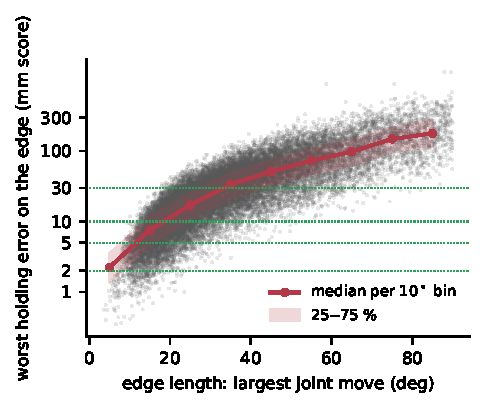
\includegraphics[width=0.52\linewidth]{figures/prm_viol_vs_length.pdf}
\caption{Worst holding error (score, Eq.~\ref{eq:score}) of every free edge of the
\PrmLargestBudget-node B18 roadmap against the edge's largest joint move. Dotted
lines: the four query tolerances.}
\label{fig:viol}
\end{figure}

Figure~\ref{fig:viol} is the single most important measurement of the pilot,
because it fixes how dense a roadmap has to be. Both ends of every edge hold the
bar exactly, yet the straight line between them does not: the median worst error
is \PrmMedianScoreShort\,mm for edges shorter than $20^\circ$ and
\PrmMedianScoreLong\,mm for edges of $60^\circ$ and more. For the short edges
that matter at small tolerances, sort the free edges by length (largest joint
move) into three narrow bins and take the median worst holding error in each:
\begin{center}
\footnotesize
\begin{tabular}{@{}lrrr@{}}
\toprule
edge length (largest joint move, deg) & 2.5--7.5 & 7.5--12.5 & 12.5--17.5 \\
free edges in the bin (count) & 51 & 642 & 2683 \\
median worst holding error (mm) & 1.0 & 3.6 & 6.9 \\
\bottomrule
\end{tabular}
\end{center}
In words: an edge of about $5^\circ$ drifts about 1\,mm from the holding surface
at its worst point; an edge as long as the continuity step $\tau = 10^\circ$
drifts about 3.6\,mm. Over this range the error grows roughly in proportion to the
length rather than with its square, so the roadmap's edges are far from the
regime where a straight chord hugs the curved holding surface. Two consequences
follow. First, a sub-2\,mm path needs a chain of edges of about $5^\circ$ each;
a roadmap sampled freely in twelve dimensions does not supply that density, so
the gaps below are best read as \emph{upper bounds} on how close a start is to
the goal set. Second, the holding error, not collision, is what limits a
joint-space roadmap: \PrmFreeEdgeShareLargest\,\% of candidate edges are
collision-free, but only 1.1\,\% of those free edges stay within 2\,mm, 7.5\,\%
within 5\,mm, 21\,\% within 10\,mm and 57\,\% within 30\,mm.

\subsection{The roadmaps and what they cost}

\begin{table}[h]
\centering
\footnotesize
\setlength{\tabcolsep}{3pt}
\caption{The four B18 roadmaps (goal-2 anchors, seed 0, 8 workers), one column
per node budget. A draw is one draw of the driving arm's six joints, followed by
one IK call for the other arm. A component is a set of nodes joined by
collision-free edges; the anchor rows say how many of the 7 goal anchors and the
73 start anchors sit in the largest one.}
\label{tab:build}
\begin{tabular}{@{}>{\raggedright\arraybackslash}p{6.8cm} rrrr@{}}
\toprule
node budget & 500 & 1000 & 2000 & 4000 \\
\midrule
sampled nodes kept: the node budget (count) & 500 & 1000 & 2000 & 4000 \\
all nodes, anchors included (count) & 581 & 1081 & 2081 & 4081 \\
driver-arm draws, one IK call each (count) & 2656 & 5344 & 10688 & 21408 \\
collision checks, sampling and edges together (count) & 11818 & 23969 & 47606 & 89047 \\
candidate edges measured (count) & 2922 & 6094 & 13028 & 26908 \\
collision-free edges (count) & 2657 & 5586 & 12000 & 25056 \\
components: separate islands of the free graph (count) & 71 & 90 & 125 & 173 \\
nodes in the largest component (count) & 262 & 525 & 1285 & 2557 \\
goal anchors in the largest component & 3 of 7 & 3 of 7 & 7 of 7 & 7 of 7 \\
start anchors in the largest component & 24 of 73 & 25 of 73 & 27 of 73 & 27 of 73 \\
\midrule
sampling time (s, wall clock) & 12 & 16 & 24 & 40 \\
edge measuring time (s, wall clock) & 28 & 74 & 103 & 181 \\
whole build (s, wall clock) & 51 & 100 & 138 & 232 \\
edge phase speed-up (worker-seconds per wall-second) & 7.4 & 7.8 & 7.9 & 8.0 \\
\bottomrule
\end{tabular}

\end{table}

\begin{figure}[h]
\centering
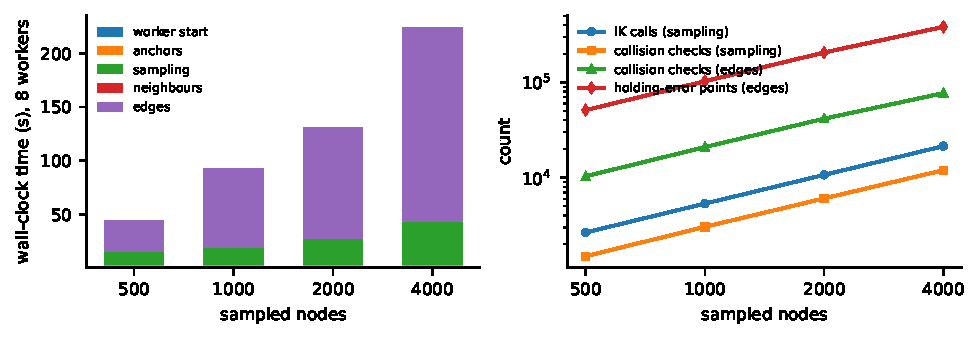
\includegraphics[width=\linewidth]{figures/prm_cost.pdf}
\caption{Left: where the build time goes. Right: the work counted, against the node budget.}
\label{fig:cost}
\end{figure}

\paragraph{Counting queries, as the meeting asked.}
Every build cost one analytical IK call per draw, and the sampler kept about one
node in four and a half draws: of the 21\,408 draws of the 4000-node build, 56\,\%
were reachable by the other arm, and 39\,\% of those were collision-free. The line
mode was by far the most productive (31\,\% of its draws kept, against 17\,\% for
the Gaussian and 5\,\% for the box), which is why it carries half the mix. The
edge phase then dominates: 77\,076 collision checks for 26\,908 edges, of which
1852 (6.9\,\%) collide. In worker time, collision checking was most of the
whole build (93\,\%: 1571 of 1680 worker-seconds at 4000 nodes, 15.7--17.9\,ms per check)
and IK 2.7\,\% (2.1\,ms per call); the 382\,241 holding-error points cost
nothing measurable. This inverts the pilot plan's expectation that IK would be
the expensive operation: here it is the full-cell compas\_fab check, exactly as
in the BiRRT's own profile. The GPU question is therefore a question about
batched collision checking, not about IK.

\paragraph{Parallel speed-up.}
Edge checking ran at 7.4--8.0 worker-seconds per wall-second on eight workers
(Table~\ref{tab:build}), i.e.\ essentially linearly; sampling reached 6.0 at 4000
nodes and less on small budgets, where a round is only a few chunks. The query's
endpoint expansion (38\,384 branch pairs collision-checked for the 807 starts)
ran at 7.2 and the endpoint edges at 7.7. The whole 4000-node build took
232\,s of wall time.

\paragraph{What an ``all-starts'' query is, and why it takes 200\,s.}
An all-starts query takes all 807 library start poses of the goal as its start
set and gives each of them an exact gap. It is a survey of the start poses, not
one planning query: on the same roadmap, the query with only starts 0 and 12
took 8.9\,s. The all-starts query took 208--229\,s whatever the roadmap size;
for the 4000-node roadmap the 212\,s split as follows.
\begin{center}
\footnotesize
\begin{tabular}{@{}>{\raggedright\arraybackslash}p{4.3cm} r >{\raggedright\arraybackslash}p{8.3cm}@{}}
\toprule
phase & time (s) & what it depends on \\
\midrule
solve and collision-check the start poses (38\,384 branch pairs) & 73 & only the start poses and the scene: can be done once and stored \\
holding error of the endpoint edges (99\,161 edges) & 28 & start poses and roadmap; not the goal \\
lazy gap verification (\PrmVerifyRounds{} rounds) & 104 & the goal; about half is the 0.64\,s spanning-tree search repeated every round, the rest is collision-checking \PrmLazyChecked{} edges (1231 blocked) \\
paths per tolerance & 3 & the goal \\
\bottomrule
\end{tabular}
\end{center}
So a night of precomputation can remove nearly all of it: with the start poses
and their edges solved and collision-checked once per roadmap, the verification
loop ends after its first round. Section~\ref{sec:precompute} builds and times
exactly this.

\paragraph{Lazy checking is exact in practice too.}
On the smoke roadmap (bar B3, 333 nodes, 380 starts) the same query was run with
endpoint edges checked lazily and eagerly: the gap of every one of the 380
starts (its smallest gap over all its branch pairs and turns) is the same both
ways, and the lazy query took 151\,s against 593\,s (two workers).

\subsection{Starts 0 and 12, and all 807 starts, against the node budget}

\begin{table}[h]
\centering
\footnotesize
\setlength{\tabcolsep}{3.5pt}
\caption{What each B18 roadmap answers, one column per node budget. The upper rows
come from the query whose start set is starts 0 and 12 only; the lower rows from
the query over all 807 starts. A gap is in mm of holding error (rotation folded
in at $0.4^\circ$ per mm); $\infty$: no route of free edges to any goal node.}
\label{tab:query}
\begin{tabular}{@{}>{\raggedright\arraybackslash}p{6.8cm} rrrr@{}}
\toprule
node budget & 500 & 1000 & 2000 & 4000 \\
\midrule
start 0: gap, best over its branch pairs and turns (mm) & 82.6 & 41.8 & 41.4 & 21.3 \\
start 0: gap of its library configuration alone (mm) & $\infty$ & $\infty$ & $\infty$ & $\infty$ \\
start 12: gap, best over its branch pairs and turns (mm) & 7.9 & 5.7 & 5.1 & 4.5 \\
start 12: gap of its library configuration alone (mm) & 22.1 & 29.2 & 29.2 & 24.2 \\
\midrule
all 807 starts: smallest gap (mm) & 7.9 & 5.7 & 4.2 & 2.9 \\
starts that reach the goal set at all (count of 807) & 650 & 657 & 657 & 657 \\
median gap of the starts that reach it (mm) & 49.4 & 41.8 & 30.5 & 24.3 \\
starts with a gap of at most 2 mm (count) & 0 & 0 & 0 & 0 \\
starts with a gap of at most 5 mm (count) & 0 & 0 & 1 & 11 \\
starts with a gap of at most 10 mm (count) & 13 & 17 & 24 & 36 \\
starts with a gap of at most 30 mm (count) & 114 & 115 & 171 & 462 \\
all-starts query time (s, wall clock) & 208 & 208 & 229 & 212 \\
\bottomrule
\end{tabular}

\end{table}

\begin{figure}[h]
\centering
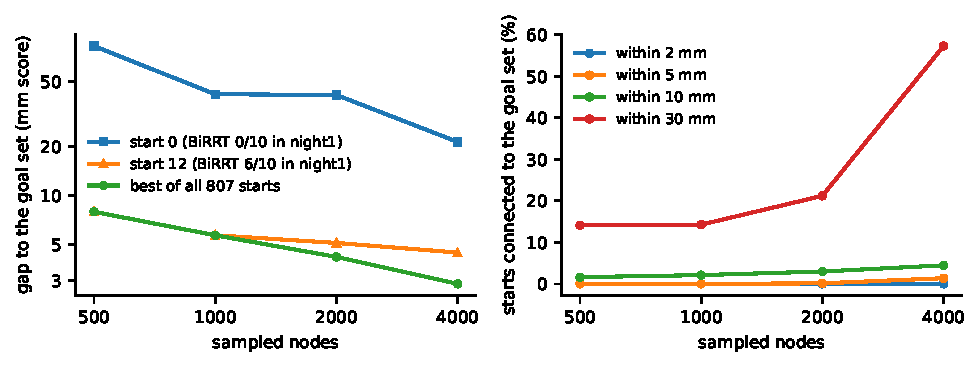
\includegraphics[width=\linewidth]{figures/prm_budget.pdf}
\caption{Left: gap to the goal set against the node budget for start 0, start 12 and
the best of all starts. Right: share of the 807 starts that reach the goal set within
each tolerance.}
\label{fig:budget}
\end{figure}

Three things stand out in Table~\ref{tab:query} and Fig.~\ref{fig:budget}.

\emph{Start 12 is near-feasible, start 0 is not.} Start 12, which the BiRRT
solved with 6 of 10 seeds in night 1, reaches the goal set within 7.9\,mm on the
smallest roadmap and within 4.5\,mm on the largest. Start 0, solved by none of
10 seeds, sits at 82.6\,mm on 500 nodes and still 21.3\,mm on 4000 nodes. The
reason is local: on the 2000-node roadmap, the 11--20 sampled nodes drawn around
start 0's two anchors ended up a median $96$--$121^\circ$ away from it (their
other arm lands on a distant IK branch, or they collide), and only two nodes lie
within $30^\circ$ of it; around start 12 the same numbers are $71$--$73^\circ$
and 13--28 nodes. Start 0's gap on that roadmap is set by three long edges
within the first five steps out of it ($45$--$52^\circ$, 31--41\,mm), not by
anything near the goal.

\emph{The library's own start configuration is often the wrong one.} For both
starts the gap of the library configuration alone (the rows ``gap of its library
configuration alone'' in Table~\ref{tab:query}) is much
larger than the best over all branch pairs and turns; for start 0 it is
unreachable at every budget. Over all starts, a different branch pair or turn
beat the library configuration for \PrmBetterBranchStarts{} of the
\PrmReachableStarts{} reachable starts, and the best node sat on the home turn
for most of them (Table~\ref{tab:turns}). This is the quantitative form of the
meeting's worry about start/goal branch pairing: fixing the start configuration
before searching throws away most of the useful connections.

\emph{More nodes help, slowly.} The best gap over all starts falls from 7.9 to
2.9\,mm from 500 to 4000 nodes, the median over starts from 49 to 24\,mm, and the
number of starts within 30\,mm from 114 to 462 (the least stable of these
numbers: Table~\ref{tab:ablation} shows it ranging from 171 to 405 across seeds
at 2000 nodes). No start reaches the goal set
within 2\,mm at any budget. Exactly the same 150 starts are unreachable at 1000,
2000 and 4000 nodes: their start nodes do have edges, but into clusters of the roadmap that no
edge of at most $90^\circ$ joins to the goal's component (the 4000-node roadmap
has 173 components); 136 of them are ``broken'' starts.

\begin{table}[h]
\centering
\footnotesize
\caption{The turn of each reachable start's best node (4000-node roadmap).}
\label{tab:turns}
\begin{tabular}{@{}lr@{}}
\toprule
turn of the best node & starts \\
\midrule
\tablerows{figures/prm_table_turns.tex}
\bottomrule
\end{tabular}
\end{table}

\subsection{Which starts are near the goal: classes, carry anchors, and the BiRRT}

\begin{table}[h]
\centering
\footnotesize
\caption{All 807 starts of B18 goal 2 on the \PrmLargestBudget-node roadmap, by the
library's straight-line class and by the BiRRT's outcome in experiment 2. ``reach'':
starts with any route to the goal set; the last four columns count starts within each
tolerance (mm).}
\label{tab:classes}
\begin{tabular}{@{}lrrrrrrr@{}}
\toprule
group & starts & reach & median gap & $\le$2 & $\le$5 & $\le$10 & $\le$30 \\
\midrule
\tablerows{figures/prm_table_classes.tex}
\bottomrule
\end{tabular}
\end{table}

\begin{table}[h]
\centering
\footnotesize
\caption{The same starts by carry anchor. The last column counts the starts of each
anchor that the BiRRT solved at least once in experiment 2.}
\label{tab:carry}
\begin{tabular}{@{}lrrrrrr@{}}
\toprule
carry anchor & starts & reach & median gap & $\le$10 & $\le$30 & BiRRT solved \\
\midrule
\tablerows{figures/prm_table_carry.tex}
\bottomrule
\end{tabular}
\end{table}

\begin{figure}[h]
\centering
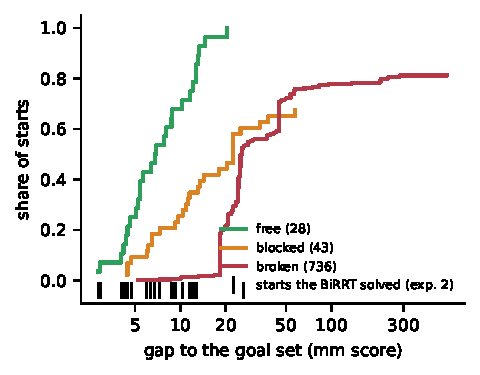
\includegraphics[width=0.52\linewidth]{figures/prm_gap_by_class.pdf}
\caption{Share of starts whose gap is below a value, per library class (starts with no
route are the missing share at the right). Ticks under the axis: the gaps of the
starts the BiRRT solved in experiment 2.}
\label{fig:classes}
\end{figure}

\paragraph{The roadmap ranks the starts the way the BiRRT did.}
The roadmap never ran the BiRRT and knows nothing about its results, yet the
starts the BiRRT solved at least once in experiment 2 are the ones the roadmap
puts closest to the goal set: all \PrmBirrtSolvedStarts{} of them are reachable,
their median gap is \PrmSolvedMedianGap\,mm against 24.3\,mm for the starts it
never solved, 15 of them are within 10\,mm and all 21 within 30\,mm
(Table~\ref{tab:classes}). The five starts with the smallest gaps were all solved
by the BiRRT, and seven of the best ten. The library's straight-line classes are
ordered the same way (medians 6.8, 11.5 and 24.4\,mm for free, blocked and
broken). The ranking is not perfect in the other direction: 21 of the 36 starts
within 10\,mm were never solved in experiment 2, but that batch ran only two seeds
per start, and one of those 21 is start 12, which night 1 solved with 6 of 10
seeds.

\paragraph{The carry anchor matters most.}
Table~\ref{tab:carry} is the clearest single result. Every start the BiRRT solved
is a ``back'' carry pose, and so is every start within 10\,mm of the goal set; no
horizontal or vertical start comes within 10\,mm, and the vertical ones have a
median gap of 57\,mm. The benchmark's night-1 analysis found that production's
start derivation always picks the horizontal anchor and succeeds 2.7\,\% of the
time from it. For this goal the roadmap says why: from a horizontal carry pose no
route of short joint-space steps reaches any of the goal's branch pairs.

\subsection{The best path}

\begin{figure}[h]
\centering
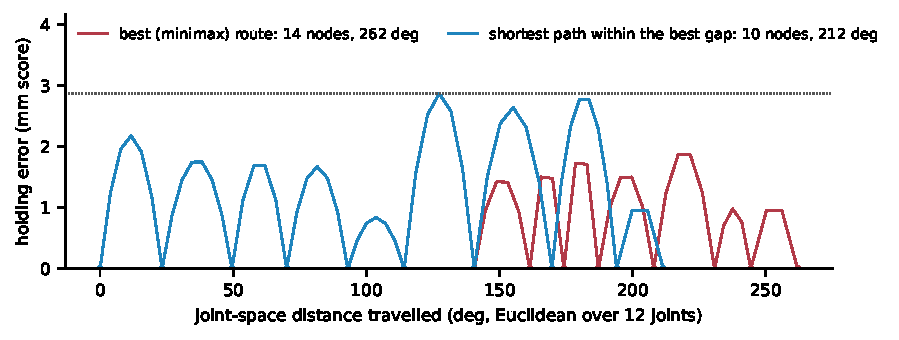
\includegraphics[width=\linewidth]{figures/prm_profile.pdf}
\caption{Holding error along the best route of the \PrmLargestBudget-node roadmap
(start \PrmBestStart) and along the shortest path within the same gap. Dots: roadmap
nodes, where the error is zero. Dotted line: the gap.}
\label{fig:profile}
\end{figure}

The best route of the \PrmLargestBudget-node roadmap starts at start
\PrmBestStart{} (a back, free-class start the BiRRT solved), on branch pair
\PrmBestStartPair{} and the \PrmBestStartTurn{} turn --- not its library
configuration --- and ends at the goal's branch pair \PrmBestGoalLibraryPair{}
(library numbering). It has \PrmBestRouteNodes{} nodes and travels
\PrmBestRouteLength\,rad in joint space, with no joint moving more than
\PrmBestRouteMaxStep$^\circ$ between the dense points of the profile, so it
contains no branch flip by construction. Its worst holding error is
\PrmBestGap\,mm. Figure~\ref{fig:profile} shows what that number is made of: the
error rises from zero at each node to a peak in the middle of each edge and
falls back to zero at the next node, and the peaks are all of similar height.
Only two of the thirteen edges peak above 2\,mm (at 2.2 and 2.9\,mm); the others
peak between 0.8 and 1.9\,mm. There is no plateau and no single dominant spike:
this is a resolution limit of the roadmap, not a sign that the start and the
goal sit on disconnected sheets. Replacing those two edges by shorter ones ---
locally resampling around them, as the plan's refinement step proposes --- is
all that stands between this route and a sub-2\,mm path. The filtered searches
tell the same story from the other side: within 5\,mm eleven starts connect, the
shortest such path (7 nodes, from start 312, another BiRRT-solved start) has a
worst error of 4.6\,mm, and within 10 and 30\,mm the shortest paths have 5--6
nodes.

\begin{figure}[h]
\centering
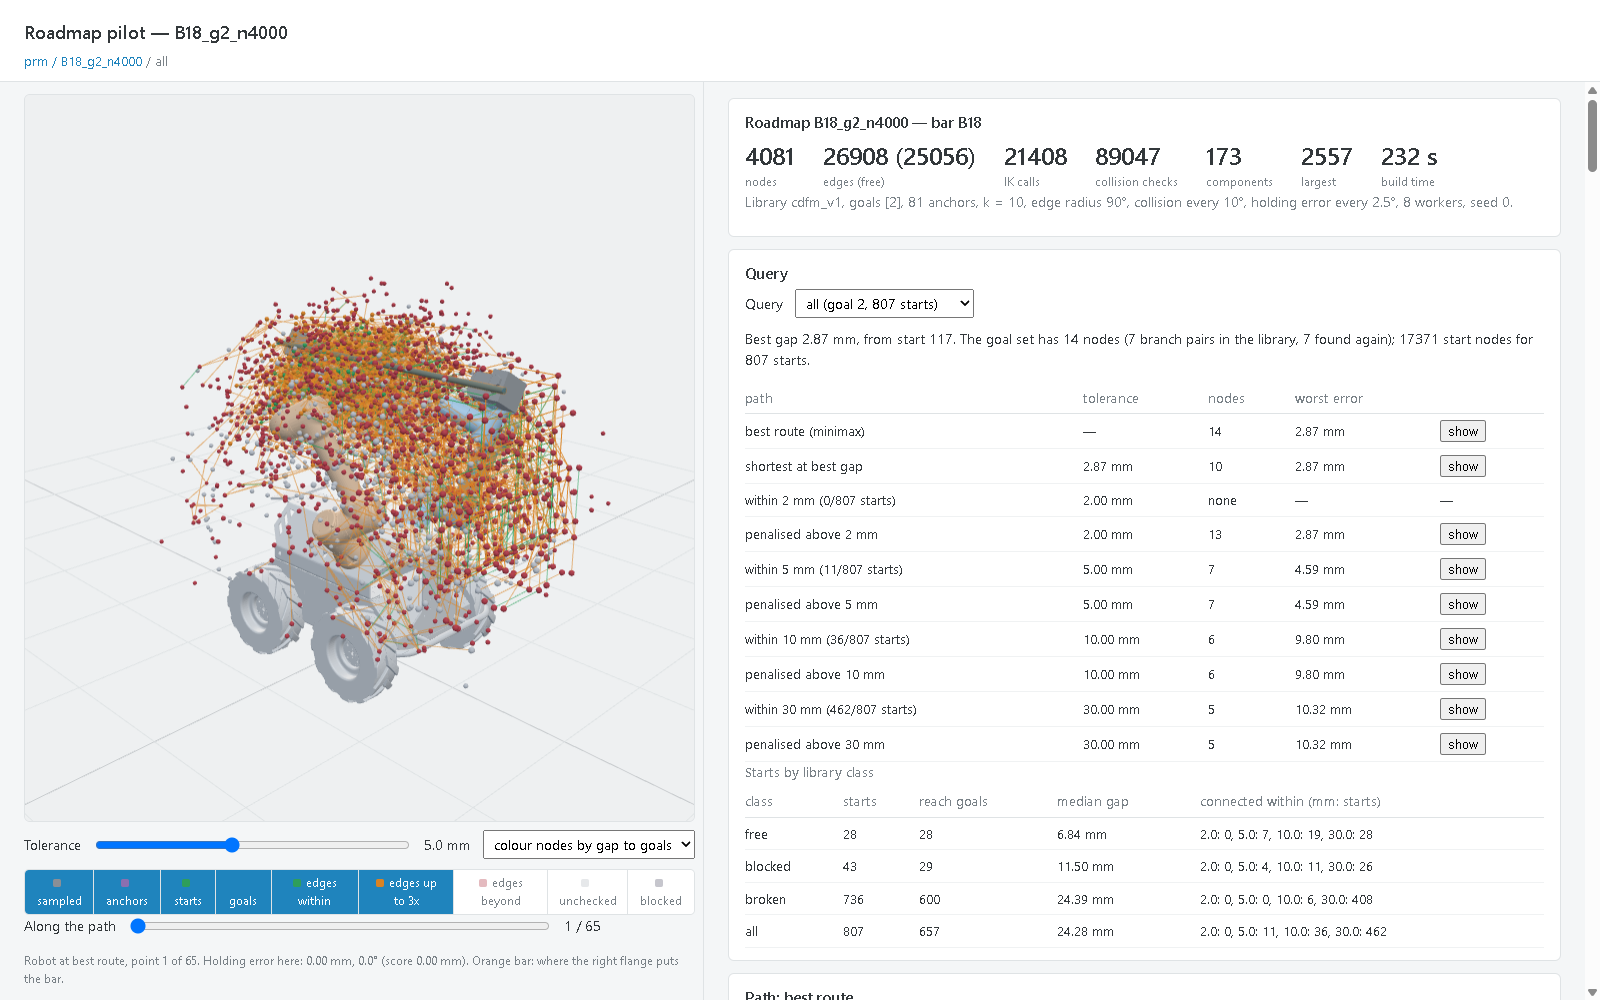
\includegraphics[width=\linewidth]{figures/prm_dashboard.png}
\caption{The roadmap page on the 4000-node B18 roadmap and the all-starts query:
nodes at the midpoint of the two flanges, coloured by their gap to the goal set at
the 5\,mm slider setting, edges coloured by their worst holding error, the robot
posed at the first point of the best route.}
\label{fig:dashboard}
\end{figure}

\subsection{Seeds and two sampler choices}

\begin{table}[h]
\centering
\footnotesize
\setlength{\tabcolsep}{3.5pt}
\caption{The 2000-node B18 roadmap under three seeds and two sampler changes, one
column per roadmap; rows as in Tables~\ref{tab:build} and~\ref{tab:query}.}
\label{tab:ablation}
\begin{tabular}{@{}>{\raggedright\arraybackslash}p{6.2cm} rrrrr@{}}
\toprule
roadmap & \shortstack{seed 0\\(default)} & seed 1 & seed 2 & \shortstack{every IK\\branch kept} & \shortstack{no line\\draws} \\
\midrule
sampled nodes kept: the node budget (count) & 2000 & 2000 & 2000 & 2000 & 2000 \\
all nodes, anchors included (count) & 2081 & 2081 & 2081 & 2081 & 2081 \\
driver-arm draws, one IK call each (count) & 10688 & 9280 & 10304 & 2272 & 16768 \\
collision checks, sampling and edges together (count) & 47606 & 46198 & 46252 & 45350 & 58085 \\
candidate edges measured (count) & 13028 & 12983 & 12896 & 9500 & 11929 \\
collision-free edges (count) & 12000 & 11871 & 11909 & 8611 & 10174 \\
components: separate islands of the free graph (count) & 125 & 139 & 148 & 296 & 200 \\
nodes in the largest component (count) & 1285 & 1044 & 1034 & 755 & 1460 \\
goal anchors in the largest component & 7 of 7 & 3 of 7 & 3 of 7 & 3 of 7 & 3 of 7 \\
start anchors in the largest component & 27 of 73 & 24 of 73 & 24 of 73 & 23 of 73 & 48 of 73 \\
\midrule
sampling time (s, wall clock) & 24 & 19 & 24 & 21 & 25 \\
edge measuring time (s, wall clock) & 103 & 82 & 98 & 78 & 97 \\
whole build (s, wall clock) & 138 & 114 & 133 & 110 & 132 \\
edge phase speed-up (worker-seconds per wall-second) & 7.9 & 7.9 & 7.9 & 7.8 & 7.9 \\
\midrule
start 0: gap, best over its branch pairs and turns (mm) & 41.4 & 33.0 & 23.5 & 73.2 & 38.2 \\
start 0: gap of its library configuration alone (mm) & $\infty$ & $\infty$ & $\infty$ & $\infty$ & $\infty$ \\
start 12: gap, best over its branch pairs and turns (mm) & 5.1 & 3.9 & 5.0 & 5.3 & 13.7 \\
start 12: gap of its library configuration alone (mm) & 29.2 & 11.2 & 34.1 & 31.1 & 29.1 \\
\midrule
all 807 starts: smallest gap (mm) & 4.2 & 3.8 & 5.0 & 5.2 & 13.7 \\
starts that reach the goal set at all (count of 807) & 657 & 651 & 658 & 658 & 650 \\
median gap of the starts that reach it (mm) & 30.5 & 24.3 & 24.5 & 44.0 & 25.5 \\
starts with a gap of at most 2 mm (count) & 0 & 0 & 0 & 0 & 0 \\
starts with a gap of at most 5 mm (count) & 1 & 4 & 3 & 0 & 0 \\
starts with a gap of at most 10 mm (count) & 24 & 25 & 27 & 16 & 0 \\
starts with a gap of at most 30 mm (count) & 171 & 400 & 405 & 112 & 406 \\
all-starts query time (s, wall clock) & 229 & 236 & 205 & 203 & 188 \\
\bottomrule
\end{tabular}

\end{table}

\paragraph{Seeds.} Across three seeds at 2000 nodes the best gap is 3.8--5.0\,mm,
start 12's gap 3.9--5.1\,mm, and 24--27 starts are within 10\,mm: these numbers
are stable. Start 0's gap (23.5--41.4\,mm) and the count within 30\,mm (171,
400, 405) are not; seed 0 happens to be the unlucky one for both, so the 30\,mm
counts of Table~\ref{tab:query} should be read with a spread of that size.

\paragraph{Keeping every IK branch} makes each draw yield more nodes, and that
is exactly why it does worse at a fixed node budget. The budget counts nodes,
not draws: 2000 nodes came from only 2272 draws (about 10\,000 with
$\beta = 1$), so four times fewer distinct bar poses were tried, and each was
copied onto postures far from each other (flipped elbows and wrists, a median
$182^\circ$ from the anchor on the smoke roadmap). Such copies find few
neighbours within $90^\circ$, so the roadmap has \emph{fewer} edges, not more
(3500 fewer), falls into 296 components, and every quality number is worse
(median gap 44\,mm, 16 starts within 10\,mm, 112 within 30\,mm). The effort is
spread over many branch sheets instead of filling the one or two that connect
the starts to the goal. Section~\ref{sec:e4} gives it the same number of draws.

\paragraph{Without the start--goal line draws} the roadmap still covers the
space (406 starts within 30\,mm, similar to the default seeds) but loses all
precision: no start comes within 10\,mm, and the best gap rises to 13.7\,mm.
This is not about the start itself. A start's gap is the worst edge anywhere
on its best route to the goal, not something measured at the start; line
draws put closely spaced nodes all along the corridor between starts and goal
pairs, and without them the middle of every route is made of long edges, and a
long edge drifts far from the holding surface (Fig.~\ref{fig:viol}). The
near-feasible routes of Fig.~\ref{fig:profile} are made almost entirely of
line-draw nodes; they are what the roadmap's precision rests on. Line draws are
also the most productive per draw (31\,\% kept, against 17\,\% for the Gaussian
and 5\,\% for the box, at 4000 nodes), which is why the no-line roadmap needed
16\,768 draws for the same 2000 nodes.

\subsection{From roadmap routes to exact paths (E2)}
\label{sec:e2}

\begin{table}[h]
\centering
\footnotesize
\setlength{\tabcolsep}{3pt}
\caption{Refinement of the all-starts queries (Section~\ref{sec:refine}), one column per
roadmap or tracker setting. ``Exact path from a route within $t$'' means: some route all
of whose roadmap edges score at most $t$ was turned into waypoints that hold the bar
exactly, are collision-free and never move a joint more than $10^\circ$.}
\label{tab:refine}
\begin{tabular}{@{}>{\raggedright\arraybackslash}p{7.6cm} rrrrr@{}}
\toprule
refinement & \shortstack{4000 nodes\\knots $2.5^\circ$} & \shortstack{4000 nodes\\end nodes only} & \shortstack{2000 nodes\\seed 0} & \shortstack{2000 nodes\\seed 1} & \shortstack{2000 nodes\\seed 2} \\
\midrule
starts within 30 mm on the roadmap: the ones refined (count) & 462 & 462 & 171 & 400 & 405 \\
edges tracked (count) & 3329 & 3388 & 1091 & 2373 & 2735 \\
\quad of which the tracker turned into exact waypoints & 2737 & 2762 & 885 & 1961 & 2304 \\
\quad failed: no IK solution at some waypoint & 65 & 45 & 14 & 35 & 37 \\
\quad failed: a joint jumped more than $10^\circ$ & 136 & 119 & 25 & 98 & 104 \\
\quad failed: a corrected waypoint collides & 19 & 47 & 1 & 16 & 21 \\
\quad failed: changes elbow branch, so it cannot meet the next edge & 372 & 415 & 166 & 263 & 269 \\
edges re-tracked from a route's last waypoint at a node (count) & 0 & 0 & 0 & 0 & 0 \\
edges dropped because a route could not continue (count) & 1 & 2 & 0 & 0 & 0 \\
\midrule
starts with an exact path from a route within 2 mm, of those the roadmap brings within 2 mm & 0 of 0 & 0 of 0 & 0 of 0 & 0 of 0 & 0 of 0 \\
starts with an exact path from a route within 5 mm, of those the roadmap brings within 5 mm & 11 of 11 & 11 of 11 & 1 of 1 & 4 of 4 & 3 of 3 \\
starts with an exact path from a route within 10 mm, of those the roadmap brings within 10 mm & 34 of 36 & 33 of 36 & 24 of 24 & 25 of 25 & 27 of 27 \\
starts with an exact path from a route within 30 mm, of those the roadmap brings within 30 mm & 245 of 462 & 169 of 462 & 81 of 171 & 81 of 400 & 129 of 405 \\
\midrule
best start: smallest exact gap (mm) & 2.87 & 2.87 & 4.20 & 3.78 & 4.97 \\
\quad its start index & 117 & 117 & 227 & 313 & 12 \\
\quad waypoints of its exact path (count) & 178 & 139 & 207 & 125 & 164 \\
\quad largest joint step between waypoints (deg) & 2.76 & 3.55 & 2.69 & 2.57 & 2.31 \\
\quad holding error of its waypoints (mm) & 4e-09 & 4e-09 & 4e-09 & 4e-09 & 4e-09 \\
refinement time (s, wall clock) & 1210 & 1085 & 483 & 858 & 902 \\
stored exact paths (one per start, plus the best and the shortest ones) passing the production repair at 2 mm steps & 249 of 249 & -- & -- & -- & -- \\
\bottomrule
\end{tabular}

\end{table}

\begin{figure}[h]
\centering
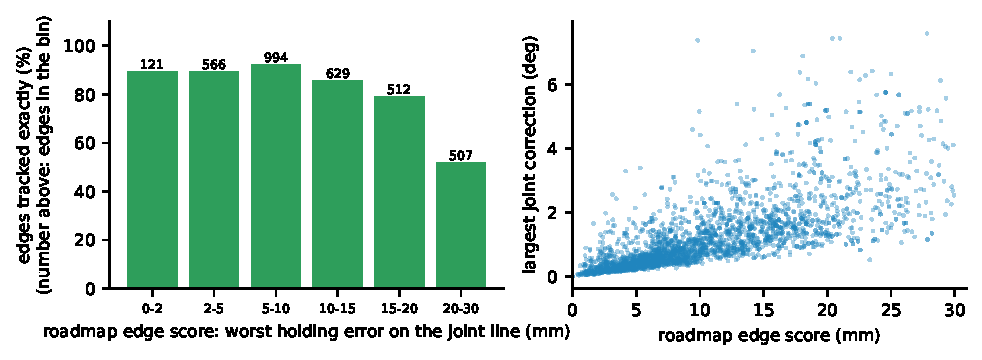
\includegraphics[width=\linewidth]{figures/prm_trackability.pdf}
\caption{Every edge the refinement of the 4000-node roadmap tracked. Left: share of
edges turned into exact waypoints, by the edge's roadmap score. Right: how far the
correction moved the joints away from the straight joint line.}
\label{fig:track}
\end{figure}

\paragraph{Within 10\,mm, almost every route becomes an exact path.} Of the
\PrmRoadmapTen{} starts the 4000-node roadmap brings within 10\,mm of the goal set,
\PrmExactTen{} have an exact path from a route within 10\,mm; within 5\,mm, all
\PrmRoadmapFive{} do; within 30\,mm, \PrmExactThirty{} of \PrmRoadmapThirty. The whole
refinement of the 807-start query took \PrmRefineSeconds\,s on eight workers
(\PrmRefineRounds{} tracking rounds, \PrmRefineEdges{} edges tracked). The best start
is the same as the roadmap's (start \PrmExactBestStart): its exact path has
\PrmExactBestWaypoints{} waypoints, holds the bar to $10^{-7}$\,m, and moves no joint
more than \PrmExactBestStep$^\circ$ between waypoints.

\paragraph{Why 10\,mm is a good working tolerance.} Fig.~\ref{fig:track} shows that an
edge's chance of tracking stays near 90\,\% up to 10\,mm (89\,\% under 5\,mm, 92\,\%
between 5 and 10\,mm; the failures there are mostly edges whose joint line passes a
stretched elbow, which no tolerance helps) and then falls: 86\,\% between 10 and
15\,mm, 79\,\% between 15 and 20\,mm, 52\,\% between 20 and 30\,mm. The joint correction
grows at about $0.1^\circ$ per mm of roadmap error (median over the tracked edges). So
up to 10\,mm the roadmap's routes are nearly as good as exact ones, and a 10\,mm roadmap
is the right thing to search before refining, as proposed. Of the \PrmRefineEdges{} tracked edges, \PrmRefineBranchChange{} changed
elbow branch, \PrmRefineContinuity{} hit the continuity gate, \PrmRefineIk{} met a pose
one arm cannot reach, and \PrmRefineCollision{} collided once corrected.

\paragraph{The same on other roadmaps, and why the knots matter.} On the three
2000-node roadmaps (seeds 0, 1, 2), every start within 10\,mm got an exact path (24 of
24, 25 of 25, 27 of 27); within 30\,mm, 81 of 171, 81 of 400 and 129 of 405
(Table~\ref{tab:refine}). So ``within 10\,mm on the roadmap'' reliably means ``an exact
path exists'', while within 30\,mm it is roughly a coin toss that depends on the
roadmap. Tracking a straight bar move between the two end nodes instead of following
the bar along the joint line (``end nodes only'') gives nearly the same answer within
10\,mm (33 of 36) but clearly fewer exact paths within 30\,mm (169 against 245): on
longer edges the bar's straight move strays further from the joint line, and more of
those edges change branch (415 against 372) or collide (47 against 19).

\paragraph{Exact paths from starts the BiRRT never solves.} \PrmExactHorizontal{}
horizontal starts have an exact path (from routes between 10 and 30\,mm), although the
BiRRT solved none of the 458 horizontal starts in experiment 2; \PrmExactBack{} back
starts do too, \PrmExactThirty{} in all, against the BiRRT's 21 (two seeds per
start). \PrmExactBirrtOverlap{} of the 21 starts the BiRRT
solved are among them. This qualifies the carry-anchor finding above: from a
horizontal carry pose no route stays within 10\,mm, but many routes within 30\,mm can
still be made exact.

\begin{table}[h]
\centering
\footnotesize
\caption{The production check of every stored exact path of the 4000-node refinement:
the production repair (\code{core.repair_joint_path}) re-solves each path at 2\,mm and
0.002\,rad bar steps with the production solver, gate and collision check.}
\label{tab:validation}
\begin{tabular}{@{}>{\raggedright\arraybackslash}p{8.0cm} rrrr@{}}
\toprule
carry anchor & back & horizontal & vertical & all \\
\midrule
starts within 30 mm on the roadmap (count) & 171 & 291 & 0 & 462 \\
starts with an exact path from the roadmap (count) & 81 & 164 & 0 & 245 \\
\quad passing the production repair at 2 mm steps & 81 & 164 & 0 & 245 \\
\quad failing it on a collision between the 1 cm waypoints & 0 & 0 & 0 & 0 \\
\quad failing it otherwise & 0 & 0 & 0 & 0 \\
\midrule
starts the BiRRT solved at least once in experiment 2 (count) & 21 & 0 & 0 & 21 \\
\quad of which the roadmap also gives a production-checked path & 20 & 0 & 0 & 20 \\
\bottomrule
\end{tabular}

\end{table}

\paragraph{The production check.} \PrmCheckPassed{} of the \PrmCheckPaths{} exact paths
pass the production repair unchanged (Table~\ref{tab:validation}; \PrmCheckSeconds\,s on
eight workers), \PrmCheckPassedHorizontal{} of them from horizontal starts and
\PrmCheckPassedBirrt{} from starts the BiRRT also solved: every path the refinement
returns is one the production planner would accept as is. Earlier versions of the
tracker passed 7 of 38, then 217 of 244, then 243 of 268 paths; the difference was
hidden branch hops near straight elbows, which the production walk at 2\,mm does not take
(Section~\ref{sec:refine}). Removing them also removes the starts whose only exact
route relied on such a hop, which is why the counts in Table~\ref{tab:refine} are
lower than in the first version (298 starts within 30\,mm then, \PrmExactThirty{} now;
within 10\,mm the count stayed at 34).

\subsection{Tightening routes: tube draws (way 2) and a seeded BiRRT (way 1) (E3)}
\label{sec:e3}

\begin{table}[h]
\centering
\footnotesize
\caption{The 4000-node refinement without and with three rounds of tube draws
(each round: 200 draws around the routes of the 20 starts with the largest exact gap
above 10\,mm).}
\label{tab:tube}
\begin{tabular}{@{}>{\raggedright\arraybackslash}p{7.4cm} rr@{}}
\toprule
refinement & without tube draws & with 3 tube rounds \\
\midrule
starts with an exact path from a route within 2 mm (count) & 0 & 20 \\
starts with an exact path from a route within 5 mm (count) & 11 & 86 \\
starts with an exact path from a route within 10 mm (count) & 34 & 120 \\
starts with an exact path from a route within 30 mm (count) & 245 & 245 \\
nodes added by tube draws (count) & 0 & 10099 \\
tube rounds run (count) & 0 & 3 \\
target starts improved, summed over rounds (count) & -- & 60 \\
refinement time (s, wall clock) & 1210 & 1888 \\
stored exact paths passing the production repair at 2 mm steps & 249 of 249 & 125 of 125 \\
\bottomrule
\end{tabular}

\end{table}

\begin{table}[h]
\centering
\footnotesize
\caption{The seeded BiRRT on the 24 starts still without any exact path after the tube
rounds (smallest roadmap gaps first; all have roadmap gaps under 30\,mm).}
\label{tab:birrt}
\IfFileExists{figures/prm_table_birrt.tex}{\begin{tabular}{@{}>{\raggedright\arraybackslash}p{7.4cm} rr@{}}
\toprule
seeded BiRRT & seeded with the exact chains & from the two ends only \\
\midrule
unresolved starts tried (count) & 24 & 24 \\
a path found (count) & 0 & 1 \\
\quad passing the production repair (count) & 0 & 1 \\
median time of a passing run (s) & -- & 15 \\
median IK solves of a passing run (count) & -- & 806 \\
of the starts tried, solved by the plain BiRRT in experiment 2 (count) & 0 & 0 \\
time limit per start (s) & 120 & 120 \\
\bottomrule
\end{tabular}
}{(missing)}
\end{table}

\paragraph{Tube draws work: the needed tolerance drops several-fold.} Drawing nodes in a
narrow tube ($5^\circ$) around a start's current route and searching again is the
refinement proposed in the meeting, and it does what was hoped
(Table~\ref{tab:tube}): with three rounds of about 3400 nodes each, the starts with an
exact path from a route within 10\,mm went from 34 to 120 (42 of them horizontal, none
before), within 5\,mm from 11 to 86, and within 2\,mm from none to 20. Every target start
improved in every round. The best route now needs only 0.89\,mm of roadmap tolerance
(start 206, whose roadmap gap was 23.4\,mm before the tubes). The tubes do not add
starts beyond the 245 that already had an exact path within 30\,mm: they tighten
routes, they do not create them. They cost 12 minutes on top of the 20-minute
refinement, and all 125 exact paths stored from the tube-refined routes pass the
production repair as well.

\paragraph{The seeded BiRRT does not bridge what the tracker cannot.} On the 24 starts
left without any exact path (Table~\ref{tab:birrt}), the BiRRT seeded with the
route's exact pieces found no path in 120\,s each; started from the two ends only,
with the same tube of samples, it found one (start 573, in 15\,s, and it passes the
production check). Of the 49 failed edges on these 24 routes, 30 are branch changes at a
stretched elbow (Section~\ref{sec:refine}) and 17 pass through poses one arm cannot
reach; a task-space tree grown from the exact pieces meets the same obstacles, so
seeding it with them does not help (it may even hurt: the trees start deep inside the
two branch sheets that do not meet). These are
the hardest starts of the goal, so the sample says little about the BiRRT in general,
but for this refinement the roadmap side (tubes) is clearly the better lever.

\subsection{Wider edges (E1) and every IK branch at the same number of draws (E4)}
\label{sec:e1}

\begin{table}[h]
\centering
\footnotesize
\setlength{\tabcolsep}{3pt}
\caption{E1: the 4000-node roadmap rebuilt with edges of up to $160^\circ$ (same
seed, so the same sampled nodes; only the edges differ). E4: every IK branch kept,
given about the same number of draws (10\,848) as the default 2000-node roadmap
(10\,688 draws, one branch per draw), next to the earlier every-branch roadmap that
stopped at 2000 nodes (2272 draws).}
\label{tab:e1e4}
\begin{tabular}{@{}>{\raggedright\arraybackslash}p{6.2cm} rrrrr@{}}
\toprule
roadmap & \shortstack{4000 nodes\\$90^\circ$ (ref.)} & \shortstack{4000 nodes\\$160^\circ$ (E1)} & \shortstack{every branch\\2272 draws} & \shortstack{every branch\\10k draws (E4)} & \shortstack{one branch\\10k draws (ref.)} \\
\midrule
sampled nodes kept: the node budget (count) & 4000 & 4000 & 2000 & 9400 & 2000 \\
all nodes, anchors included (count) & 4081 & 4081 & 2081 & 9481 & 2081 \\
driver-arm draws, one IK call each (count) & 21408 & 21408 & 2272 & 10848 & 10688 \\
collision checks, sampling and edges together (count) & 89047 & 101487 & 45350 & 232212 & 47606 \\
candidate edges measured (count) & 26908 & 29089 & 9500 & 56748 & 13028 \\
collision-free edges (count) & 25056 & 25928 & 8611 & 51717 & 12000 \\
components: separate islands of the free graph (count) & 173 & 68 & 296 & 533 & 125 \\
nodes in the largest component (count) & 2557 & 3873 & 755 & 5839 & 1285 \\
goal anchors in the largest component & 7 of 7 & 7 of 7 & 3 of 7 & 3 of 7 & 7 of 7 \\
start anchors in the largest component & 27 of 73 & 67 of 73 & 23 of 73 & 49 of 73 & 27 of 73 \\
\midrule
sampling time (s, wall clock) & 40 & 35 & 21 & 99 & 24 \\
edge measuring time (s, wall clock) & 181 & 226 & 78 & 658 & 103 \\
whole build (s, wall clock) & 232 & 272 & 110 & 769 & 138 \\
edge phase speed-up (worker-seconds per wall-second) & 8.0 & 6.0 & 7.8 & 6.0 & 7.9 \\
\midrule
start 0: gap, best over its branch pairs and turns (mm) & 21.3 & 21.3 & 73.2 & 21.8 & 41.4 \\
start 0: gap of its library configuration alone (mm) & $\infty$ & 648.9 & $\infty$ & $\infty$ & $\infty$ \\
start 12: gap, best over its branch pairs and turns (mm) & 4.5 & 4.5 & 5.3 & 4.3 & 5.1 \\
start 12: gap of its library configuration alone (mm) & 24.2 & 24.2 & 31.1 & 24.2 & 29.2 \\
\midrule
all 807 starts: smallest gap (mm) & 2.9 & 2.9 & 5.2 & 3.4 & 4.2 \\
starts that reach the goal set at all (count of 807) & 657 & 801 & 658 & 713 & 657 \\
median gap of the starts that reach it (mm) & 24.3 & 25.0 & 44.0 & 23.1 & 30.5 \\
starts with a gap of at most 2 mm (count) & 0 & 0 & 0 & 0 & 0 \\
starts with a gap of at most 5 mm (count) & 11 & 11 & 0 & 12 & 1 \\
starts with a gap of at most 10 mm (count) & 36 & 36 & 16 & 47 & 24 \\
starts with a gap of at most 30 mm (count) & 462 & 462 & 112 & 471 & 171 \\
all-starts query time (s, wall clock) & 212 & 553 & 203 & 340 & 229 \\
\bottomrule
\end{tabular}

\end{table}

\paragraph{E1: $160^\circ$ edges connect more starts, but only through useless
edges.} Widening the edge limit from $90^\circ$ to $160^\circ$ merged the roadmap
from 173 components into 68 and made 801 of the 807 starts reachable instead of
657. But the 144 newly reachable starts reach the goal set only through edges that
break the holding constraint by 220 to 1787\,mm (median 984\,mm; none within
100\,mm): a straight joint line of more than $90^\circ$ simply does not hold the bar.
Of the 657 starts reachable both ways, 11 got a smaller gap, all of them above
30\,mm before and after. Nothing within 30\,mm changed (best gap 2.87\,mm; 11, 36
and 462 starts within 5, 10 and 30\,mm), while the all-starts query took 553\,s
instead of 212\,s (272 verification rounds instead of 80). The $90^\circ$ limit
was not hiding useful connections; the islands it leaves apart are joined only by
moves no path can use.
\label{sec:e4}

\paragraph{E4: every IK branch is worth it per draw, not per second.} With the node
budget counting nodes, keeping every branch looked worse (Table~\ref{tab:ablation}).
Given the same number of draws as the one-branch roadmap, it is clearly better: 47
starts within 10\,mm and 471 within 30\,mm, against 24--27 and 171--405 for the three
one-branch seeds, and a best gap of 3.4\,mm against 3.8--5.0\,mm. That is about what
the one-branch roadmap reaches with twice the draws (4000 nodes: 36 and 462). But it
has 9481 nodes, 56\,748 candidate edges and 232\,000 collision checks, and took
769\,s to build against 232\,s for the 4000-node one-branch roadmap; its graph is
also more broken (533 components, only 3 of the 7 goal anchors in the largest).
Per collision check the one-branch roadmap is still ahead: 36 starts within 10\,mm
for 89\,000 checks, against 47 for 232\,000. The other branches help because they
are other routes to the same goal pairs, which is also the motivation for the
start and goal \emph{sets}.

\subsection{Re-calibrating the three carry poses (E5)}
\label{sec:e5}

The library's start poses come from three carry anchors that were never
calibrated; the horizontal one, for example, puts the grasp midpoint at
$x = 0.40$\,m, 19\,cm closer to the robot than the demo pose it was taken from.
The search (\path{holding_prm/carry.py}, \path{scripts/prm_carry_search.py})
keeps the three classes and their bar axes (horizontal: along $y$; vertical:
along $z$; back: along $x$) and varies the rest: the grasp midpoint on a 10\,cm
grid over a $0.6 \times 0.6 \times 0.6$\,m box per class, and the roll about the
bar in $30^\circ$ steps (4116 candidates per class). A carry pose is stored as
these three numbers, so the same pose applies to any bar (the bar's orientation
follows from its grasps, as the planner's anchors do).
\begin{itemize}[nosep]
  \item \emph{Stage 1}, on bars B18 and B3: the candidate must be holdable on both
        bars; then ranked by how many of its branch pairs are comfortable (at least
        $29^\circ$ from every joint limit, and elbow and wrist at least $30^\circ$
        from straight), and by how many of 24 nudges (5\,cm and 10\,cm shifts,
        $15^\circ$ and $30^\circ$ turns, about each base axis) it survives. A pose
        close to the robot body loses its nudges toward the body. The 30 best of each
        class, spread over places and rolls, plus today's anchors, got the nudges.
  \item \emph{Stage 2}: the 5 best of each class and today's three anchors were
        given to the roadmap as the start set, against 8 goals of B18 and 6 of B3,
        one 3000-node roadmap per goal (a first try with one 4000-node roadmap over
        8 goals was too sparse: 311 components), each query refined to exact paths.
\end{itemize}

\begin{table}[h]
\centering
\footnotesize
\setlength{\tabcolsep}{3pt}
\caption{The carry search, one column per class. Midpoints in the mobile-base frame;
``goals with an exact path'' count, over the 14 goals of stage 2, those the carry pose
reaches with a path that holds the bar exactly.}
\label{tab:carrysearch}
\begin{tabular}{@{}>{\raggedright\arraybackslash}p{6.0cm} rrr@{}}
\toprule
carry class & back & horizontal & vertical \\
\midrule
grid candidates holdable on both bars (of 4116 per class) & 1277 & 2569 & 370 \\
\midrule
today's anchor at its best roll: grasp midpoint (m), roll & (0.10, 0.00, 1.04), $-60^\circ$ & (0.40, -0.04, 0.86), $-60^\circ$ & (0.71, 0.00, 0.70), $-60^\circ$ \\
\quad nudges survived on its worst bar & 24 of 24 & 24 of 24 & 23 of 24 \\
\quad goals with an exact path from a route within 10 mm (of 14) & 4 & 0 & 0 \\
\quad goals with any exact path (route within 30 mm) & 6 & 0 & 0 \\
\midrule
best candidate: grasp midpoint (m), roll & (0.00, -0.10, 1.10), $-30^\circ$ & (0.45, 0.10, 1.20), $60^\circ$ & (0.80, 0.00, 0.60), $0^\circ$ \\
\quad nudges survived on its worst bar & 24 of 24 & 24 of 24 & 20 of 24 \\
\quad goals with an exact path from a route within 10 mm (of 14) & 4 & 2 & 0 \\
\quad goals with any exact path (route within 30 mm) & 5 & 4 & 1 \\
\quad median exact gap where it has one (mm) & 5.6 & 11.6 & 19.9 \\
\bottomrule
\end{tabular}

\end{table}

\begin{figure}[h]
\centering
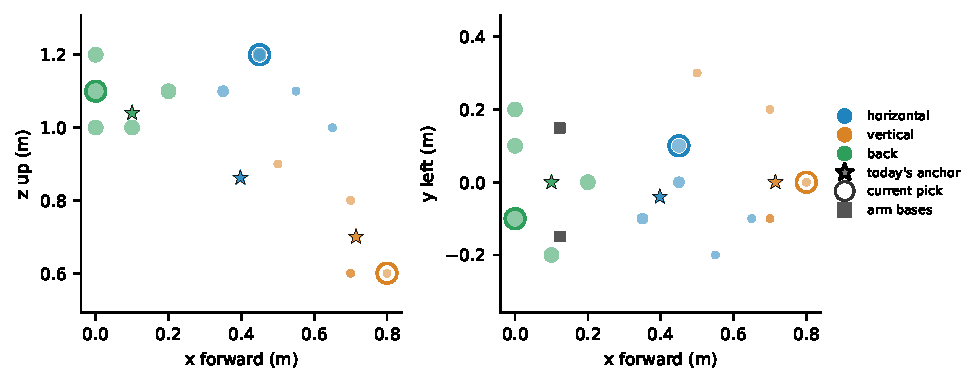
\includegraphics[width=\linewidth]{figures/prm_carry.pdf}
\caption{Stage-2 carry candidates by their grasp midpoint (side and top view; marker
size grows with the number of goals reached within 10\,mm). Stars: today's anchors;
rings: the current picks.}
\label{fig:carry}
\end{figure}

\paragraph{What the search says.} The carry \emph{class} matters more than the
exact place. Back carry is the best class: today's back anchor and the best back
candidate both reach 4 of the 14 goals with an exact path from a route within
10\,mm; moving it does not help much (the best candidate has a smaller median exact
gap, 5.6\,mm). Horizontal carry is where today's anchor is clearly wrong: it reaches
none of the 14 goals, while the best candidate, raised to $z = 1.2$\,m and moved
forward and left (midpoint $(0.45, 0.10, 1.20)$\,m, roll $60^\circ$), reaches 2
within 10\,mm and 4 with some exact path. No vertical pose works: the best reaches one
goal at 20\,mm. And for most goals no carry pose of any class reaches within 10\,mm on a
3000-node roadmap, which says the goals, not the carry poses, are the hard part at this
density. The current picks are in \path{asset/carry_poses.json}, marked
provisional, with the three best of each class listed for a person to choose from;
nothing in the planner or the library uses them yet.

\subsection{Precomputing overnight (E6)}
\label{sec:precompute}

The night before, only the bar and its grasps are known; the goal (the base's
parked pose relative to the structure) is known only on site. Everything that does
not depend on the goal can therefore move to the night: the roadmap itself, with
the three carry poses' branch pairs as nodes and every edge collision-checked, and
the exact tracking of every roadmap edge within 10\,mm (\code{prm_pilot.py track},
which writes the verdicts and waypoints to \path{tracked_10mm.json.gz}). Online, a
query only solves the goal pose and the three carry poses, measures their edges,
and searches; the refinement then tracks only the few edges that touch the goal
(\code{refine --pretracked}). The test uses goals the roadmap was \emph{not}
anchored on (B18 goals 2, 10, 20, 31, 47) and the provisional carry poses.

\begin{table}[h]
\centering
\footnotesize
\setlength{\tabcolsep}{3pt}
\caption{A night roadmap of 6000 nodes anchored on 17 other goals of B18 and the three
carry poses, then five online queries for unseen goals (8 workers). Worker start-up is
listed apart: a planner that runs for a whole session pays it once.}
\label{tab:precompute6k}
\begin{tabular}{@{}>{\raggedright\arraybackslash}p{6.4cm} rrrrr@{}}
\toprule
unseen goal & 2 & 10 & 20 & 31 & 47 \\
\midrule
night: nodes, of which anchors (count) & 6248, 248 &  &  &  &  \\
night: goals the roadmap is anchored on (count) & 17 &  &  &  &  \\
night: build time (s) & 821 &  &  &  &  \\
night: collision-free edges, of which within 10 mm (count) & 33582, 1218 &  &  &  &  \\
night: tracking the edges within 10 mm (s) & 151 &  &  &  &  \\
night: components of the free graph (count) & 318 &  &  &  &  \\
\midrule
online query: start the workers (s) & 9.8 & 10.0 & 9.6 & 10.0 & 10.0 \\
\quad solve the goal and the 3 carry poses (s) & 1.5 & 1.4 & 1.5 & 1.4 & 1.4 \\
\quad holding error of their edges (s) & 0.2 & 0.8 & 0.2 & 0.5 & 0.0 \\
\quad gaps, with lazy collision checks (s) & 0.1 & 0.2 & 0.1 & 0.3 & 0.1 \\
\quad whole query (s) & 16.5 & 16.4 & 15.4 & 15.9 & 15.2 \\
online refinement with the night's verdicts (s) & 12.0 & 12.1 & 11.6 & 11.7 & 12.1 \\
\quad of which starting its workers (s) & 9.9 & 10.1 & 9.7 & 9.8 & 10.0 \\
\midrule
best gap from the carry poses to the goal (mm) & 56.2 & 16.6 & 32.5 & 19.0 & $\infty$ \\
carry poses with an exact path within 10 mm (of 3) & 0 & 0 & 0 & 0 & 0 \\
\bottomrule
\end{tabular}

\end{table}

\paragraph{Online time is small; coverage is the problem.} Without the 10\,s of
worker start-up, an online query for an unseen goal took about 6\,s (most of it
reading the roadmap file; solving the 4 poses took 1.5\,s, the gaps 0.1--0.3\,s)
and the refinement about 2\,s (Table~\ref{tab:precompute6k}). But none of the five
unseen goals came within 10\,mm of a carry pose: best gaps of 17--56\,mm, and no
route at all to goal 47. A 6000-node roadmap spread over 17 goals is far sparser per
goal than the 4000 nodes the goal-2 roadmap spent on one goal, and only 1218 of its
33\,582 free edges are within 10\,mm. What the night has to buy is density, not
speed: Table~\ref{tab:precompute30k} repeats the test with a 30\,000-node roadmap
anchored on 45 goals.

\begin{table}[h]
\centering
\footnotesize
\setlength{\tabcolsep}{3pt}
\caption{The same test with a night roadmap of 30\,000 nodes anchored on the 45 other
goals of B18.}
\label{tab:precompute30k}
\IfFileExists{figures/prm_table_precompute_30k.tex}{\begin{tabular}{@{}>{\raggedright\arraybackslash}p{6.4cm} rrrrr@{}}
\toprule
unseen goal & 2 & 10 & 20 & 31 & 47 \\
\midrule
night: nodes, of which anchors (count) & 30494, 494 &  &  &  &  \\
night: goals the roadmap is anchored on (count) & 45 &  &  &  &  \\
night: build time (s) & 2128 &  &  &  &  \\
night: collision-free edges, of which within 10 mm (count) & 190571, 16883 &  &  &  &  \\
night: tracking the edges within 10 mm (s) & 5319 &  &  &  &  \\
night: components of the free graph (count) & 682 &  &  &  &  \\
\midrule
online query: start the workers (s) & 7.7 & 7.9 & 7.7 & 7.5 & 7.7 \\
\quad solve the goal and the 3 carry poses (s) & 1.3 & 1.1 & 1.4 & 1.2 & 1.2 \\
\quad holding error of their edges (s) & 0.3 & 0.5 & 0.3 & 0.3 & 0.0 \\
\quad gaps, with lazy collision checks (s) & 0.3 & 0.2 & 0.2 & 0.2 & 0.9 \\
\quad whole query (s) & 17.4 & 16.5 & 16.4 & 16.5 & 15.7 \\
online refinement with the night's verdicts (s) & 13.7 & 16.1 & 12.4 & 12.5 & 12.1 \\
\quad of which starting its workers (s) & 8.0 & 7.7 & 7.8 & 7.7 & 7.5 \\
\midrule
best gap from the carry poses to the goal (mm) & 40.2 & 9.8 & 11.7 & 13.1 & $\infty$ \\
carry poses with an exact path within 10 mm (of 3) & 0 & 1 & 0 & 0 & 0 \\
\bottomrule
\end{tabular}
}{(still running)}
\end{table}

\paragraph{A night-sized roadmap: closer, and the carry set becomes the limit.} The
30\,000-node roadmap took 35 minutes to build and 89 minutes to track its 16\,883 edges
within 10\,mm (16\,013 track), about two hours in all on eight workers; its largest
component holds 320 of the 405 goal anchors and 85 of the 88 carry-pose anchors. The
online cost stayed about the same (Table~\ref{tab:precompute30k}): about 16\,s per query,
of which 8\,s start the workers, 2\,s are the query's own phases and most of the rest is
reading the five-times larger roadmap file -- both would be paid once by a planner that
keeps its workers and the roadmap loaded for the session. Unseen goal 10 now has an
exact path (from a 9.8\,mm route; it passes the production repair), goals 20 and 31 come
within 12--13\,mm, goal 2 stays at 40\,mm and goal 47 has no route. Goal 2 is telling: the
all-starts query of Section~\ref{sec:e2} found routes of 2.9\,mm to it from the library's
back starts, but from the three fixed carry poses the best is 40\,mm. Fixing a single pose
per class gives up most of the start-set freedom that made the roadmap work; a small
family of carry poses per class (a few places and rolls), all in the night roadmap and
all in the online start set, costs nothing online and is the obvious next step.

\subsection{Bar B3}

\begin{table}[h]
\centering
\footnotesize
\caption{Bar B3, one 2000-node roadmap anchored on goals 4, 11 and 16; the three
night-1 starts of each goal. ``night 1'': seeds (of 10) the BiRRT solved.}
\label{tab:b3}
\begin{tabular}{@{}rrllrrrr@{}}
\toprule
goal & start & carry & class & night 1 & gap & lib. gap & best pair \\
\midrule
\tablerows{figures/prm_table_b3.tex}
\bottomrule
\end{tabular}
\end{table}

On bar B3 the roadmap orders the three night-1 starts of each goal as the BiRRT
did (Table~\ref{tab:b3}). In goal 4, start 42 (8 of 10 seeds) has a 6.5\,mm gap,
start 13 (4 of 10) 16.2\,mm, and start 0 (0 of 10) no route at all. In goal 16
the best-solved start (13, 8 of 10 seeds) has the smallest gap, 7.5\,mm, against
17.1\,mm for the other two. In goal 11, where starts 13 and 221 were each solved
twice, start 13 has 7.6\,mm and start 221 16.7\,mm. Start 0 --- production's
horizontal pick in all three goals --- has the largest gap or ties for it. Again the library configuration is rarely the best:
start 13 of goal 11 reaches the goals within 7.6\,mm on its best branch pair
but only within 35.6\,mm on its library configuration.

\subsection{What this says, and what it does not}

\paragraph{Observations.}
\begin{enumerate}[nosep,label=(\roman*)]
  \item \textbf{The pilot's two questions have first answers.} (1) On B18 goal 2,
        a joint-continuous path exists whose holding error stays under
        \PrmBestGap\,mm, from a start the BiRRT also solved, found with 4000
        nodes: 23\,024 IK calls (21\,408 to build, 1616 to solve the 808 endpoint
        poses) and 141\,501 collision checks (89\,047 to build, 52\,454 for the
        query over all 807 starts), in 232\,s plus 212\,s on eight workers. No
        path under 2\,mm was found at any budget. (2) Where the
        roadmap fails, the failure is local and of known shape: the best route's
        error is a row of similar peaks at 1--3\,mm, two edges over 2\,mm; start
        0's is a few long edges right next to the start.
  \item \textbf{The gap is a useful difficulty measure without running the BiRRT.}
        It separates the starts the BiRRT solved from those it did not
        (median 6.8 against 24.3\,mm), orders the library's classes, and on B3
        orders the night-1 starts of three goals as the BiRRT did.
  \item \textbf{The carry anchor, and the branch pair, are decided wrongly today.}
        For B18 goal 2 only back-carry starts come within 10\,mm, while
        production picks the horizontal anchor; and for 610 of 657 reachable
        starts some other branch pair or turn beats the library's own start
        configuration. A roadmap query over a set of starts makes both choices
        by search.
  \item \textbf{Global density is the wrong lever.} Doubling the node budget
        from 2000 to 4000 lowered the best gap from 4.2 to 2.9\,mm and did not
        reach any start that was unreachable at 1000. The holding error of an
        edge is set by its length (Fig.~\ref{fig:viol}), and random nodes do
        not shorten the edges of one particular route fast enough.
  \item \textbf{Collision checking is the cost.} 93\,\% of build worker time;
        IK is under 3\,\%. The work parallelises almost perfectly on the CPU
        (8.0x on 8 workers for edges). A GPU, if ever, would be for batched
        collision checks.
\end{enumerate}

\paragraph{What the numbers do not say.}
A gap is an upper bound on the smallest holding error a path needs: a denser or
better-placed roadmap can only lower it. ``Unreachable'' means unreachable in
this roadmap within $90^\circ$ edges, not infeasible ($90^\circ$ is the
largest move of any single joint along one edge, in either direction, so a
band of $180^\circ$; Section~\ref{sec:e1} widens it to $160^\circ$). Each budget was built once
(seed 0); at 2000 nodes a different seed moves the best gap by about 1\,mm and
the 30\,mm count by more than a factor of two (Table~\ref{tab:ablation}). Collision along an edge is checked every $10^\circ$ of joint motion,
coarser than the production planner's 2\,mm pose steps, so a roadmap path has
to be re-solved exactly (\code{core.repair_joint_path}, step 7 of the plan)
before it can be executed; the pilot does not do this yet. And all of this is
one goal of one bar, plus three goals of B3.

\paragraph{Second version: what the new experiments add.}
\begin{enumerate}[nosep,label=(\roman*),resume]
  \item \textbf{A 10\,mm roadmap route is nearly an exact path.} Tracking the bar
        along a route and solving both arms at every step turned 34 of the 36 routes
        within 10\,mm, and 245 of 462 within 30\,mm, into exact paths; all 245 pass
        the production repair unchanged. That is about twelve times the 21 starts the BiRRT
        solved, including 164 horizontal starts it never solved (Section~\ref{sec:e2}).
  \item \textbf{The hard part of exactness is branches, not millimetres.} Most
        edges that fail to track have a joint line through a stretched elbow, where
        the exact path ends on the mirror branch; and four rounds of the production
        check were needed to find every way a coarse chain can hop between branches
        near such a point (Section~\ref{sec:refine}).
  \item \textbf{Wider edges do not help; more branches help per draw}
        (Section~\ref{sec:e1}).
  \item \textbf{Carry poses: the class matters more than the place.} Back carry is
        best and today's back anchor is about as good as any; today's horizontal
        anchor reaches none of 14 goals, a raised one reaches 2--4; no vertical pose
        works (Section~\ref{sec:e5}).
  \item \textbf{Overnight precomputation makes the online part a few seconds}, but
        the night has to buy density: a 6000-node roadmap over 17 goals reached none
        of 5 unseen goals within 10\,mm (Section~\ref{sec:precompute}).
\end{enumerate}

\paragraph{Next steps suggested by the data.}
\begin{enumerate}[nosep]
  \item \textbf{Bring the refinement into the planner}: a \code{use_prm} variant of
        \code{plan_constrained_dual_arm} that queries a stored roadmap with the carry
        poses as the start set, refines, and hands the production repair a path, and
        a benchmark variant so it can be batched against the BiRRT.
  \item \textbf{Collision distance along the route}: the production check passes
        everything now, but only collisions at 1\,cm waypoints are checked during
        tracking; a clearance cost would keep routes away from contact.
  \item \textbf{Denser night roadmaps}: decide the node budget per goal region from
        the 30\,000-node test, and whether goals of one structure can share it.
  \item \textbf{Choose the carry poses} from the three listed per class, then
        re-run the night build with them.
\end{enumerate}


% Third part of holding_prm_report.tex (input from there): the roadmap as a
% backend of plan_constrained_dual_arm, used in scenes that change from bar to bar.
% Tables come from docs/figures/make_prm_figures.py (robarch_* functions).

% =============================================================================
\section{A precomputed roadmap behind \texttt{plan\_constrained\_dual\_arm}, in a changing scene}
\label{sec:scene}
% =============================================================================

Sections~\ref{sec:build}--\ref{sec:refine} built and refined roadmaps inside the
benchmark's scenes, which hold only the robot, its tools and the carried bar. On
site the scene is different for every bar: the bars built so far, their joints,
and sometimes a support robot stand around the goal, and the base parks a few
centimetres off its planned pose. This section puts the roadmap behind the
production entry point and makes it work there. The idea is the one from the
meeting notes: \emph{precompute} a roadmap per bar that knows only the robot, its
tools and the bar; \emph{online}, place it at the real base pose and check only
what the precompute could not know.

\subsection{What is reused, and what has to be redone}

\begin{center}
\footnotesize
\begin{tabular}{@{}p{4.6cm} p{5.0cm} p{5.6cm}@{}}
\toprule
 & depends on & online \\
\midrule
roadmap nodes and edges & the bar, its two grasps & reused as they are \\
collisions among robot, tools, bar and the joint halves on the bar & the same & reused (verdicts of the precompute) \\
exact waypoints of each edge (tracking) & the same & reused \\
the goal as seen from the robot & base pose, goal in the world & solved fresh: a few IK calls \\
collisions with built bars, joints, support robots & base pose, the scene & checked fresh, only on what a route uses \\
\bottomrule
\end{tabular}
\end{center}

\noindent
A node is twelve joint values, so it does not depend on where the base stands;
neither does anything that rides on the arms. The roadmap is therefore built once,
\emph{in the robot's frame}, and ``moving it to the real base pose'' needs no
computation on the roadmap at all: the planner reads the two arm bases from the
live scene and expresses the world goal with them,
\[
  {}^{\text{base}}T_{\text{bar}}^{\text{goal}} \;=\;
  \bigl({}^{\text{world}}T_{\text{base}}\bigr)^{-1}\; {}^{\text{world}}T_{\text{bar}}^{\text{goal}} .
\]
A base parked elsewhere moves the goal as seen from the robot, and moves the
scene; nothing else. There is one roadmap per bar, never several to stitch.

\subsection{Splitting the collision check}
\label{sec:split}

The production check (\code{planner.check_collision} of compas\_fab) tests
everything against everything in one call and has no per-body filter. The split
is made by editing a private copy of the cell state, so compas\_fab itself is
unchanged (\code{sampling.make_collision_fns}):

\begin{description}[nosep,leftmargin=1.5em]
  \item[full] the production check, as before.
  \item[robot side] every body and tool that does not ride on the robot is hidden.
        What is left is exactly what the precompute scene tests.
  \item[scene only] every carried body is allowed to touch all robot links, all
        other carried bodies and the arm tools; the arm tools are allowed to touch
        all robot links; and the robot's self-collision pass is skipped. What is
        left is robot links, tools and carried bodies against the bodies and tools
        standing in the scene. Allowances the design authored toward the scene
        (the bar may touch the joint halves it will sit in) are kept.
\end{description}

\noindent
Two facts make the reuse sound, and both are tested on a real scene (the last
test of \path{test_holding_prm.py}): the full check says
``collides'' exactly when the robot-side check or the scene-only check does; and
the precompute scene, with the base at the origin and nothing built, gives the
same verdict as the robot-side check in the real scene at the real base pose.
Table~\ref{tab:robarchsplit} gives the result and the time of each check.

\paragraph{A signature guards the reuse.} The robot-side verdicts are valid only
for the same load. The roadmap stores a signature of what they depend on (the
bar, every carried body with its link, attachment frame and allowed contacts
among the carried bodies, the arm tools' allowed links); the planner compares it
with the live start state and the caller's right-hand grasp, and stops with
\code{RoadmapMismatch}, listing the differences, when they do not match. A
roadmap built from a benchmark library has no signature and is refused. There
is no fallback to another roadmap or to the BiRRT.

\subsection{Precompute for one exported bar}

\code{prm_pilot.py build --problem-dir <export> --bar B4} builds the roadmap of
one bar from the exported action files, in the trimmed scene of
\code{benchmark build-cells} (robot, tools, the bar and its joint halves).

\begin{description}[nosep,leftmargin=1.5em]
  \item[goal anchors] the planned goal pose of the carry movement
        (\code{target_ee_frames} of the jointing file, seen from the planned base
        pose), plus the same world goal seen from 12 bases shifted by up to
        10\,cm and turned by up to $5^\circ$ (\code{--base-error-m},
        \code{--base-error-deg}, \code{--base-samples}). Each pose is expanded to
        all its collision-free branch pairs. The roadmap is then dense around a
        goal \emph{region}, so that the real goal, which will coincide with none of
        the 13, has neighbours.
  \item[start anchors] the 18 carry poses of the family found in
        Section~\ref{sec:e5} (\path{prm/carry/carry_v1/starts.json}), every
        branch pair.
  \item[the rest] sampling, edges and exact tracking of every edge within 15\,mm
        (\code{prm_pilot.py track}), as in Sections~\ref{sec:build}
        and~\ref{sec:refine}.
\end{description}

\subsection{The online plan}
\label{sec:online}

\begin{algo}{\textsc{PlanOnRoadmap} --- \texttt{online.plan\_on\_roadmap}}{alg:online}
\Function{PlanOnRoadmap}{live scene and start state, world goal pose of the bar, roadmap folder}
  \State load the roadmap; \textbf{stop} unless its signature matches the load in the scene \Comment{no fallback}
  \State read the arm bases from the live scene; check numpy FK against the simulator ($10^{-5}$\,m)
  \State workers: this process (1 worker), or $n$ processes that open the scene from files
         \Comment{cell cached by geometry}
  \State $G \gets$ every collision-free branch pair at the goal pose \Comment{full check, in the scene}
  \State $S \gets$ the roadmap's carry-pose nodes that pass the scene-only check
  \State join new goal nodes to their nearest roadmap nodes; load the night's tracking verdicts
  \For{tolerance $t$ in 10, 20, 30\,mm}
    \Loop
      \State route $\gets$ shortest route $S \to G$ over edges within $t$ not known bad; \textbf{break} if none
      \State edges tracked overnight: scene-only check of their stored waypoints \Comment{parallel, lazy}
      \State other edges (they touch a new goal node): track now, full check \Comment{parallel}
      \State drop the edges that failed; \textbf{continue} unless the whole route is usable
      \State join the edges' waypoints into one exact path \Comment{Section~\ref{sec:refine}}
      \State walk it at the caller's step (2\,mm) and full-check every fine waypoint \Comment{parallel}
      \State \Return the fine path if clean; else drop the edge that failed and \textbf{continue}
    \EndLoop
  \EndFor
  \State one tube round around the best route left (Section~\ref{sec:refine}), then the loop once more
  \State \Return failure, with the smallest tolerance a remaining route would need
\EndFunction
\end{algo}

\noindent
The scene check is \emph{lazy}: only edges on a candidate route are checked, and
only against the scene, because their robot side was settled overnight. An edge
keeps a separate chain of waypoints for each direction; a direction that touches
the scene is dropped on its own. The final check replaces the production repair
of Section~\ref{sec:refine} (which ran in one process and took 30--190\,s per
path): the same fine walk and the same collision check, spread over the workers,
and a failure costs one edge and another search round rather than the plan.

\paragraph{A new base pose, or a newly built bar.} Nothing in the roadmap is
redone. The goal nodes are solved again (the goal moved as seen from the robot)
and joined to the roadmap; scene verdicts are asked again, lazily. The cached
scene files are keyed by the scene's geometry, so a new base pose rewrites only
the small state file, not the cell.

\subsection{Switching planners}

\code{plan_constrained_dual_arm} keeps its signature and gains two keywords:
\code{backend="birrt"} (default, unchanged) or \code{"prm"}, and
\code{prm_options} (\code{roadmap_dir}, \code{workers}, \code{tolerances_mm},
\code{tube_rounds}). The roadmap branch returns the same \code{(path, info)}; an
unknown backend, a missing roadmap or a roadmap for another load raise. After
the roadmap plan the path goes through the same optional repair and the same
shortcut smoothing as a BiRRT path.

\code{scripts/headless_bar_action_planner.py} plans the bar carry of an exported
jointing file with either planner:
\begin{quote}\footnotesize
\code{headless_bar_action_planner.py <data> --problem 260920_RobArch_demo_revamp}\\
\hspace*{1.5em}\code{--bar-action B4__J.json --movement cdfm --cdfm-backend prm --prm-workers 8}
\end{quote}
(\code{--movement cdfm} finds the carry by its type and reads home from the
release file; \code{--prm-run} names another roadmap than
\code{<problem>__<bar>}; \code{--save-tag} and \code{--save-dir} keep results of
different runs apart; \code{--base-shift} plans as if the base parked off its
planned pose.) \code{scripts/prm_check_solved.py} then checks a saved path on its
own: production repair at 2\,mm with the calibrated solver, the $10^\circ$ gate
and the full collision check in the scene of the saved start state.

\paragraph{Looking at a plan.} Two ways. \code{--replay-file <saved motion file> --gui}
replays any saved path in the planner script's PyBullet window, in the scene of the
saved start state, with a slider along the path. And every online plan is saved as a
query of its roadmap (\path{prm/<run>/queries/<bar>_<tag>.json.gz}, with the scene
it was planned in): after \code{prm_pilot.py export --name <run>}, which also writes
the robot's and the scene's 3D files, the roadmap page
(\path{http://localhost:8000/prm/<run>/dashboard/} over a web server on the data root)
draws the built bars, joint halves and support robots around the robot, marks the
edges the scene blocked, and walks the plan's exact path with its stepper; the
holding error it measures along that path is zero. Under the stepper the page
plots, for the exact path or for a node's best route alike, the holding error at
the commanded points (one dot per point, so the density of the data is visible),
the holding error along a dense joint-space interpolation of the same path
($0.1^\circ$ per joint, the step of the planner's own path checker), which
approximates what the robot shows while its controller tracks the path between
commanded points, and the twelve joint angles along the path. On the exact B4 path
(1525 points, at most $0.3^\circ$ between neighbours) the dense interpolation adds
nothing measurable; on a node route interpolated at the roadmap's $2.5^\circ$ it
rises by a few hundredths of a millimetre over the value at the points.

\subsection{Test bed: B1, B3 and B4 of the RobArch demo export}
\label{sec:scenetest}

The three bars are the first three the two-arm robot carries in
\path{data_design_study/260920_RobArch_demo_revamp}; their scenes grow as the
structure does (Table~\ref{tab:robarchpre}). The movement planned is the bar carry
embedded in each jointing file (movement \code{J_M3}, the constrained two-arm
free movement), from a carry pose the planner
chooses to the authored goal pose, any arm posture.

\begin{table}[h]
\centering
\footnotesize
\setlength{\tabcolsep}{4pt}
\caption{The three bars, their scenes at carry time, and the roadmap precomputed for
each (6000 sampled nodes plus anchors; 8 workers). B3's and B4's tracking ran while
other jobs used the machine; B1's times are from an idle machine.}
\label{tab:robarchpre}
\IfFileExists{figures/prm_table_robarch_precompute.tex}{\begin{tabular}{@{}>{\raggedright\arraybackslash}p{7.4cm} rrr@{}}
\toprule
bar & B1 & B3 & B4 \\
\midrule
bar length (m) & 1.80 & 2.00 & 0.70 \\
bodies riding on the arms: bar and joint halves (count) & 9 & 8 & 3 \\
scene at carry time: built bars and joint halves (count) & 0 & 9 & 17 \\
scene at carry time: support robots (count) & 2 & 2 & 2 \\
\midrule
goal poses the arms can hold: planned + 12 shifted bases & 11 of 13 & 13 of 13 & 13 of 13 \\
carry poses the arms can hold & 10 of 18 & 18 of 18 & 17 of 18 \\
nodes (count) & 6352 & 6460 & 6342 \\
collision-free edges (count) & 35461 & 34668 & 38689 \\
components of the free graph (count) & 243 & 302 & 224 \\
goal nodes in the largest component & 52 of 154 & 55 of 206 & 30 of 96 \\
carry-pose nodes in the largest component & 54 of 197 & 101 of 253 & 112 of 245 \\
\midrule
build: sampling and edges (s) & 641 & 631 & 490 \\
build: workers & 8 & 8 & 8 \\
edges within 15 mm, tracked exactly (count) & 4094 & 8260 & 12849 \\
\quad of which track & 3720 & 7930 & 12567 \\
tracking (s) & 1556 & 3691 & 6860 \\
\bottomrule
\end{tabular}
}{(missing)}
\end{table}

\begin{table}[h]
\centering
\footnotesize
\setlength{\tabcolsep}{4pt}
\caption{The roadmap planner on the bar carry of each bar, in its real scene, with 8
workers (\code{--cdfm-backend prm}). Times are wall-clock seconds on an otherwise
idle machine; ``worker-seconds'' add up the time inside all workers.}
\label{tab:robarchplans}
\IfFileExists{figures/prm_table_robarch_plans.tex}{\begin{tabular}{@{}>{\raggedright\arraybackslash}p{7.4cm} rrr@{}}
\toprule
bar & B1 & B3 & B4 \\
\midrule
result: tolerance of the route used & 20 mm & 20 mm & 10 mm \\
carry-pose nodes free in the scene & 197 of 197 & 248 of 253 & 245 of 245 \\
carry pose the route starts from & horizontal\_1 & horizontal\_4 & vertical\_4 \\
nodes on the route; waypoints returned (count) & 7; 824 & 7; 760 & 10; 1323 \\
edges looked at, of which usable (count) & 6, 6 & 6, 6 & 23, 14 \\
\quad blocked by the scene (count) & 0 & 0 & 9 \\
\quad dropped in the final check (count) & 0 & 0 & 0 \\
tube rounds needed (count) & 0 & 0 & 0 \\
scene-only checks: count, worker-seconds & 373, 3.1 & 349, 4.7 & 1187, 17.7 \\
full checks: count, worker-seconds & 998, 26.3 & 1478, 45.8 & 1421, 41.6 \\
\midrule
start the workers (s) & 15.4 & 17.0 & 15.2 \\
read the roadmap; write or find the scene files (s) & 0.7 & 0.8 & 0.7 \\
goal postures and carry-pose nodes in the scene (s) & 1.5 & 2.9 & 3.6 \\
search: scene checks and tracking of route edges (s) & 6.5 & 6.9 & 3.2 \\
final check at 2 mm (s) & 4.2 & 8.4 & 7.3 \\
roadmap plan in all (s) & 28.4 & 36.0 & 30.1 \\
smoothing afterwards, in the caller's process (s) & 57.4 & 44.5 & 30.1 \\
whole planning call (s) & 88.9 & 83.6 & 63.3 \\
\midrule
independent check of the saved path & pass & pass & pass \\
path length: bar travel (m); bar turning (deg) & 1.44; 70 & 1.13; 109 & 1.17; 158 \\
path length: joint travel (deg) & 140 & 146 & 190 \\
lowest point of bar, joints and tools on the path (m) & -0.003 & 0.048 & 0.071 \\
\quad the same at the goal itself (m) & -0.003 & 0.048 & 0.071 \\
\bottomrule
\end{tabular}
}{(missing)}
\end{table}

\begin{table}[h]
\centering
\footnotesize
\setlength{\tabcolsep}{4pt}
\caption{The BiRRT on the same three movements (three runs each; a run may use up to
five attempts of 300\,s), the roadmap planner with 8 workers and with one, and the
roadmap planner without the night's tracking file. ``fail (t)'': no path after
$t$ seconds.}
\label{tab:robarchcompare}
\IfFileExists{figures/prm_table_robarch_compare.tex}{\begin{tabular}{@{}>{\raggedright\arraybackslash}p{7.4cm} rrr@{}}
\toprule
bar & B1 & B3 & B4 \\
\midrule
BiRRT: runs solved (of 3) & 3 & 3 & 3 \\
BiRRT: whole planning call of each run (s) & 183, 188, 185 & 64, 65, 63 & 1624, 504, 397 \\
BiRRT: solved paths that pass the independent check & 3 of 3 & 3 of 3 & 3 of 3 \\
BiRRT: lowest point on its paths (m) & -0.003 & 0.048 & 0.071 \\
BiRRT: bar travel of each path (m) & 0.41, 0.51, 0.41 & 1.15, 1.15, 1.15 & 1.49, 2.06, 2.51 \\
BiRRT: joint travel of each path (deg) & 128, 217, 126 & 144, 144, 144 & 570, 563, 779 \\
\midrule
roadmap, 8 workers: whole planning call (s) & 89 & 84 & 63 \\
\quad of which the roadmap plan (s) & 28 & 36 & 30 \\
\quad of which starting the workers (s) & 15 & 17 & 15 \\
roadmap, 1 worker: whole planning call (s) & 78 & 116 & 118 \\
\quad of which the roadmap plan (s) & 57 & 86 & 93 \\
\midrule
roadmap, 8 workers: search with the night's tracking (s) & 7 & 7 & 3 \\
roadmap, 8 workers: search without it (s) & 6 & 12 & 16 \\
\quad roadmap plan without it (s) & 27 & 38 & 41 \\
\bottomrule
\end{tabular}
}{(missing)}
\end{table}

\begin{table}[h]
\centering
\footnotesize
\setlength{\tabcolsep}{4pt}
\caption{The base parked off its planned pose (shift in the base's own frame, then a
turn about its vertical axis). Each cell: the tolerance of the route used, the time
of the roadmap plan, and the independent check of the saved path.}
\label{tab:robarchshift}
\IfFileExists{figures/prm_table_robarch_shift.tex}{\begin{tabular}{@{}>{\raggedright\arraybackslash}p{5.0cm} rrr@{}}
\toprule
base shift & B1 & B3 & B4 \\
\midrule
5 cm forward, $+3^\circ$ & 20 mm, 30 s, pass & 20 mm, 35 s, pass & 10 mm, 42 s, pass \\
5 cm back-right, $-3^\circ$ & 20 mm, 28 s, pass & 10 mm, 33 s, pass & 10 mm, 30 s, pass \\
10 cm left, $+5^\circ$ & 20 mm, 29 s, pass & 20 mm, 32 s, pass & 10 mm, 50 s, pass \\
10 cm back-left, $-5^\circ$ & goal unholdable & 20 mm, 33 s, pass & 10 mm, 34 s, pass \\
\bottomrule
\end{tabular}
}{(missing)}
\end{table}

\begin{table}[h]
\centering
\footnotesize
\setlength{\tabcolsep}{4pt}
\caption{One collision check of each kind, on 252 configurations spread between home
and the goal posture (one process, idle machine), and whether the split agrees with
the full check.}
\label{tab:robarchsplit}
\IfFileExists{figures/prm_table_robarch_split.tex}{\begin{tabular}{@{}>{\raggedright\arraybackslash}p{7.4cm} rrr@{}}
\toprule
bar & B1 & B3 & B4 \\
\midrule
full check, real scene (ms) & 21.1 & 23.3 & 22.0 \\
scene-only check, real scene (ms) & 7.2 & 10.6 & 11.1 \\
robot-side check, real scene (ms) & 20.1 & 18.8 & 18.1 \\
full check, precompute scene (ms) & 18.5 & 17.2 & 15.1 \\
\midrule
test configurations colliding: full check (of 252) & 45 & 84 & 109 \\
\quad robot side & 45 & 51 & 56 \\
\quad scene only & 0 & 47 & 63 \\
verdicts where the split disagrees with the full check & 0 of 252 & 0 of 252 & 0 of 252 \\
\bottomrule
\end{tabular}
}{(missing)}
\end{table}

\begin{table}[h]
\centering
\footnotesize
\setlength{\tabcolsep}{4pt}
\caption{Every saved path at its waypoints and between them
(\code{prm_check_solved.py --holding-only}). ``Between'': the path interpolated
straight in joint space at $0.1^\circ$ per joint, as the controller moves between
waypoints. The holding error is the planner's own measure (the larger of the two
``where the other flange should be'' gaps). Joint reversals: how often any joint
turns back, moves under $0.2^\circ$ ignored. Ranges over the paths of a row.}
\label{tab:robarchdense}
\IfFileExists{figures/prm_table_robarch_dense.tex}{\begin{tabular}{@{}llrrrrrrr@{}}
\toprule
bar & paths & count & \shortstack[r]{waypoints\\(count)} & \shortstack[r]{largest joint\\step (deg)} & \shortstack[r]{holding error at\\waypoints (mm)} & \shortstack[r]{holding error\\between (mm)} & \shortstack[r]{rotation\\between (deg)} & \shortstack[r]{joint\\reversals} \\
\midrule
B1 & roadmap, planned base & 3 & 824--918 & 0.30--0.31 & 0.0010--0.0016 & 0.0014--0.0023 & 0.0001 & 3 \\
B1 & roadmap, shifted bases & 3 & 789--1008 & 0.27--0.43 & 0.0005--0.0015 & 0.0012--0.0023 & 0.0001 & 0--2 \\
B1 & BiRRT & 3 & 295--346 & 0.54--1.49 & 0.0008 & 0.0064--0.0404 & 0.0004--0.0014 & 3--6 \\
\midrule
B3 & roadmap, planned base & 3 & 755--1343 & 0.28--0.74 & 0.0007--0.0008 & 0.0016--0.0044 & 0.0000--0.0001 & 0--2 \\
B3 & roadmap, shifted bases & 4 & 846--1786 & 0.25--0.51 & 0.0008--0.0020 & 0.0011--0.0033 & 0.0001 & 0--1 \\
B3 & BiRRT & 3 & 579 & 0.49 & 0.0008 & 0.0018 & 0.0001 & 0 \\
\midrule
B4 & roadmap, planned base & 3 & 1276--1515 & 0.30 & 0.0010--0.0011 & 0.0013--0.0017 & 0.0001 & 0 \\
B4 & roadmap, shifted bases & 4 & 648--2990 & 0.24--0.36 & 0.0010--0.0016 & 0.0014--0.0023 & 0.0001--0.0002 & 0--2 \\
B4 & BiRRT & 3 & 1319--1450 & 1.09--5.01 & 0.0013 & 0.0103--0.0781 & 0.0012--0.0071 & 15--31 \\
\bottomrule
\end{tabular}
}{(missing)}
\end{table}

\subsection{What was measured}

All times below are from runs made one at a time on an otherwise idle machine
(16 logical cores). A first pass ran next to the roadmap precompute and was two to
four times slower; its summaries are kept in
\path{prm/robarch_plans/shared_machine_run/} and are not used here, except where
said.

\paragraph{The roadmap precompute (T1).} A 6000-node roadmap takes 8--11 minutes to
build per bar on eight workers and 26 minutes (B1, 4094 edges) to 114 minutes
(B4, 12\,849 edges) to track; B3's and B4's tracking ran next to other jobs, so their
times in Table~\ref{tab:robarchpre} are upper bounds (at B1's rate B4 would take
about 80 minutes). All 13 goal poses can be held for B3 and B4 and 11 of 13 for B1;
of the 18 carry poses, 18 (B3), 17 (B4) and 10 (B1) can be held. B1 is the long bar
grasped far apart, and the family was found on other bars; ten poses were enough
here, so the per-bar carry search that was planned as a fallback was not needed.
The free graph is in a few hundred pieces with roughly a third of the goal nodes
in the largest one, as in Section~\ref{sec:data}.

\paragraph{The collision split holds, and the scene part is the cheap part (T4).}
On 252 configurations per bar the split agreed with the full check every time, in
both senses of Section~\ref{sec:split} (Table~\ref{tab:robarchsplit}). A scene-only
check costs 7--11\,ms against 21--23\,ms for the full check: the pairs it skips
(robot against itself, against its tools and against its load) are most of the
work. In B4's scene 63 of the 252 configurations touch the built structure and 56
collide on the robot's own side, so neither part is negligible there; in B1's
scene nothing touches the scene at all.

\paragraph{Every bar gets a path, and every path passes the independent check (T2).}
Table~\ref{tab:robarchplans} lists the roadmap planner's runs. In each scene nearly
all carry-pose nodes are free (the carry poses are held close to the robot, away
from the structure), a route within 10\,mm (B4) or 20\,mm (B1, B3) exists without any
tube round, and the fine check at 2\,mm found nothing the 1\,cm waypoints had
missed. For B4 the scene removed 9 of the 23 edges the search asked about, and the
search went around them; for B1 and B3 the first route was clean. The tolerance
only says which roadmap edges the route used: the returned path holds the bar
exactly (the bar slips at most 0.004\,mm in the right hand, measured on the saved
joints). Of the 30 plans made on the idle machine (three planner settings and four
shifted bases per bar with the roadmap, three BiRRT runs per bar), 29 returned a
path, and all 29 passed \code{prm_check_solved.py}; the thirtieth is a goal that
cannot be held (below).

\paragraph{Against the BiRRT (T2).} Table~\ref{tab:robarchcompare}. The three bars
are three different cases for the BiRRT, and its log says which:
\begin{description}[nosep,leftmargin=1.5em]
  \item[B1] The BiRRT's start derivation tracks backward from the goal toward its
        home anchors; for B1 it reached none of them in its three 40\,s shares and
        returned a \emph{partial} start 0.41\,m from the goal, leaving the rest to
        another movement. Its path is therefore 0.41--0.51\,m of bar travel, after
        183--188\,s. The roadmap planner returns a whole path from a carry pose
        (1.44\,m of bar travel) in 89\,s, of which 28\,s is planning.
  \item[B3] The straight track from the horizontal home anchor to the goal is
        collision-free, so the BiRRT skips its search and returns in 63--65\,s. The
        roadmap planner takes 84\,s (36\,s of planning, 45\,s of smoothing) for a
        path of the same length. Nothing to gain here.
  \item[B4] The BiRRT has to search between the built bars: 397, 504 and
        1624\,s (the last after four failed attempts of five minutes); in the
        first pass, on the busy machine, one of three runs failed outright after
        28 minutes. Its paths are long: 1.5--2.5\,m of bar travel and
        560--780$^\circ$ of joint travel. The roadmap planner's whole call takes
        63\,s and its path has 1.17\,m and 190$^\circ$.
\end{description}

\paragraph{Where the roadmap planner's time goes (T2, T5).} With eight workers the
roadmap plan takes 28--36\,s, and 15--17\,s of that is starting the workers (each
process loads the scene from files; a planner that keeps its workers for a session
would pay it once). The search takes 3--7\,s and the fine check 4--8\,s. Writing the
scene files the first time a structure is seen cost another 14--22\,s in earlier
runs; a new base pose rewrites only the small state file. With one worker
everything runs in the caller's process on the whole 92-body cell: 57--93\,s. The
shortcut smoothing that follows, the same code as after the BiRRT, runs in the
caller's process and takes another 17--57\,s; it is the largest single part of the
call (its time budget is only looked at between shortcut attempts, each of which
re-solves and re-checks the rest of the path).

\paragraph{The night's tracking saved little here (T4).} Without the tracking file
the search tracks its route edges online and takes 6--16\,s instead of 3--7\,s
(Table~\ref{tab:robarchcompare}): the first or second route worked in every case, so
only 6 to 23 edges were ever asked about, and eight workers track those in a few
seconds. Tracking every edge within 15\,mm in advance is the most expensive part of
the precompute (26--114 minutes) and bought at most 13\,s online. It would matter
when many routes have to be tried; on these three bars, building the roadmap
alone would have been enough.

\paragraph{A base parked off its planned pose (T3).} Table~\ref{tab:robarchshift}:
11 of the 12 shifted bases were planned in 28--50\,s with the same roadmaps, and all
11 paths pass the independent check. The goal seen from a shifted base is a new
pose; its postures became new nodes (4 to 18 per plan) joined to the roadmap, and
only the edges at those nodes had to be tracked online. The one failure is B1
with the base 10\,cm back-left and turned $-5^\circ$: no arm posture can hold the
bar at the goal from there (\code{prm_goal_unholdable}), which no planner can fix;
two of B1's 13 precomputed goal poses had the same problem.

\paragraph{Between the waypoints, and what the joints do (added 2026-10-13).}
Table~\ref{tab:robarchdense} looks at the 29 saved paths the way the roadmap page
now draws them. Every path holds the bar at its waypoints to within
0.002\,mm, whichever planner made it; that is the IK's own precision. Between the
waypoints, where the controller moves the joints in straight lines, the roadmap
paths stay within 0.005\,mm: their waypoints are the 2\,mm fine walk, at most
$0.74^\circ$ apart on any joint, and a straight joint move that short bends the
bar's pose by nothing measurable. The BiRRT paths, whose smoothing leaves steps of
up to $5^\circ$, reach 0.078\,mm and $0.007^\circ$ between waypoints (B4, third
run); twenty times what the roadmap paths show, and still a hundredth of the
loosest tolerance any route here used. Two things follow. The
holding constraint does not need the 2\,mm cut: a path with $1^\circ$ joint steps
would hold the bar to a few hundredths of a millimetre, so the fine check's cost
(Section~\ref{sec:online}) is paid for the collision check, not for holding.
And the joint evolution separates the planners more than the holding error does:
on the roadmap paths a joint turns back 0--3 times per path (moves under
$0.2^\circ$ ignored), the BiRRT's B4 paths turn back 15--31 times, with every
joint taking part (its B1 and B3 paths, which it did not have to search for,
turn back 0--6 times). A shortcut smoother removes detours but not the
zig-zag of the tree's branches, which is what the 560--780$^\circ$ of joint
travel on B4 are made of. On a finer band ($0.006^\circ$) the roadmap paths show
15--74 reversals of a few thousandths of a degree, the IK's noise on a path cut
every 2\,mm; harmless, but a joint-space smoother could take them out.

\paragraph{A note on the export.} The design was exported again on 2026-10-05 and
its cell now holds a ground slab (\code{ground_WG0}, top face at $z=-0.016$\,m).
Paths planned since then see it as a stationary body in the scene check; the
paths above predate it and were measured by completing their saved start state
with the slab's state from the current export (\code{prm_check_solved.py} says so
in its record). The lowest point of any of them, 0.031\,m, stays above it.

\subsection{What this says, and what is still open}

\begin{enumerate}[nosep,label=(\roman*)]
  \item \textbf{The scheme works as proposed.} A roadmap that knows only the robot,
        its tools and the bar is reused across base poses and scenes with no
        recomputation; the scene costs a few hundred to a thousand cheap checks per
        plan, spread over the workers.
  \item \textbf{It pays where the BiRRT has to search.} On B4 the roadmap planner's
        whole call is 6--26 times shorter than the BiRRT's and its path has a quarter
        to a third of the joint travel; on B3, where the BiRRT finds a straight
        track, the BiRRT is the quicker one; on B1 the roadmap planner returns a
        whole path where the BiRRT returns part of one.
  \item \textbf{Both planners end on another arm posture than the export's.} The
        script hands the goal over as two flange frames, so either planner picks
        the posture: the roadmap paths end $155$--$205^\circ$ (largest joint) from the
        authored \code{target_configuration}, the BiRRT paths $203$--$298^\circ$. The
        movements after the carry were authored from that configuration and must
        be re-solved, or the goal restricted to the authored posture
        (\code{goal_conf}, which \code{plan_on_roadmap} accepts; the headless script
        does not pass it yet).
  \item \textbf{No planner checked the floor on these paths.} The cell of
        2026-10-02 had no ground body. The lowest point of the bar, the joint
        halves and the tools was at the goal itself on every path from the
        planned base pose (B1's ground joint lands at $z = -0.003$\,m by design).
        Two shifted-base paths of B4 went lower than their goal: to 0.058\,m and to
        0.031\,m, against 0.071\,m at the goal. The export of 2026-10-05 added a
        ground slab, so plans made since then check against it; whether a floor
        rule is still wanted in the planners (a slab only catches the bodies the
        collision check knows) is to be decided.
  \item \textbf{The holding constraint is kept far inside tolerance, between the
        waypoints too.} At most 0.005\,mm between the waypoints of a roadmap path
        and 0.078\,mm of a BiRRT path (Table~\ref{tab:robarchdense}); the 2\,mm cut
        is for the collision check. The roadmap paths are monotone joint by joint,
        the BiRRT's searched paths are not.
  \item \textbf{Start-up and smoothing now dominate.} Keeping the workers (and the
        roadmap) alive across bars would remove 15\,s per plan; the smoothing is
        shared with the BiRRT and would need its own look.
  \item \textbf{The precompute is per bar and per grasp}, and its expensive half
        (tracking) was not needed on these bars. A build alone is 8--11 minutes per
        bar on eight workers; the node budget and the 15\,mm tracking limit have not
        been tuned.
  \item \textbf{Three bars are a small sample.} They are the first three of one
        structure; later bars carry into denser scenes, where more routes will be
        blocked and the tracking may earn its cost.
\end{enumerate}


% =============================================================================
\section{Reading guide}
\label{sec:reading}
% =============================================================================

Line numbers are from the tree as written on 30 September 2026.

\begin{center}
\footnotesize
\begin{tabular}{@{}p{6.0cm} p{5.6cm} p{3.6cm}@{}}
\toprule
read & at & this report \\
\midrule
\code{violation_from_tools}, \code{holding_violation} & \code{holding.py:295}, \code{:320} & Alg.~\ref{alg:viol} \\
\code{pose_gap} & \code{holding.py:130} & the angle \\
\code{interpolate_confs}, \code{rebranch12} & \code{holding.py:387}, \code{:421} & continuity; turns \\
\code{make_collision_fn} & \code{sampling.py:68} & collision \\
\code{arm_branches} & \code{sampling.py:148} & IK on the cached base \\
\code{draw_driver}, \code{lift_draw}, \code{sample_chunk} & \code{sampling.py:278}, \code{:323}, \code{:362} & Algs.~\ref{alg:draw}, \ref{alg:sample} \\
\code{expand_bar_pose} & \code{sampling.py:413} & Alg.~\ref{alg:expand} \\
\code{candidate_pairs}, \code{evaluate_edge}, \code{edge_cost} & \code{roadmap.py:55}, \code{:163}, \code{:209} & Alg.~\ref{alg:edge} \\
\code{minimax_to_goals}, \code{lazy_search} & \code{search.py:169}, \code{:222} & Algs.~\ref{alg:minimax}, \ref{alg:lazy} \\
\code{WorkerPool.run}, \code{init_worker} & \code{parallel.py:229}, \code{:56} & Section~\ref{sec:parallel} \\
\code{make_anchors}, \code{build_roadmap} & \code{pilot.py:289}, \code{:409} & Alg.~\ref{alg:build} \\
\code{query_roadmap} & \code{pilot.py:617} & Alg.~\ref{alg:query} \\
\bottomrule
\end{tabular}
\end{center}

\end{document}
